\chapter {Боричев Ток и сад Кучинского}

От верхней площадки фуникулера обратимся к сев\-е\-ро-западу, в сторону огромного, колонного, серокаменного здания МИД. Считается, что на его месте князь Владимир разместил пантеон языческих идолов с Перуном во главе, а после, крестившись и приняв имя Василия, низвергнул идолов и возвел там в честь святого Василия деревянную церковь, которую затем снесли, да восстановили уже каменной в 1695 году под названием Трехсвятительской. В 1888-м она вновь стала Васильевской. Однако после Батыя церковь, заложенная Владимиром, была разрушена. На том ли самом месте ее возродили в 1695? У меня есть сомнение в точности местоположения, однако будем считать, что идолы стояли если не там, то в окрестностях.

Ипатьевский список повествует:

\begin{quotation}
И нача княжити Володимер в Киеве един, и постави кумиры на холму вне двора теремного: Перуна деревяна, а голова его сребрена, а ус золот, и Хорса, и Дажьбога, и Стрибога, и Семаргла, и Мокошь. И жряху им, наричуще богы, и привожаху сыны своя и дщери, и жряху бесом, и оскверняху землю требами своими, и осквернися требами (кровьми в Лаврентьевском списке) земля Руска и холм т. Но преблагий Бог не хотяй смерти грешником; на том холме ныне церкы есть святаго Василья [...]

и постави церковь святаго Василья на холме, идеже стояша кумири Перун и прочии, идеже требы творяху князь и людье;
\end{quotation}

Два источника дополняют сказанное сообщением, что место, где Владимир ставил кумиров, находилось над Боричевым (или Буричевым) потоком.

Из поучения «Слово о идолех Владимировых»: 

\begin{quotation}
В первых постави началнейшаго кумира, именем Перуна бога грому и молнию и облаков дождевых на пригорку высоком над Буричевым потоком подобию члвечку. Тулов его бе от древа хитростне изсечен главу имущь слияну от сребра уши златы нозе железны. В руках же держаше камен по подобию Перуна палающа. Рубинами. И каръбуклем украшен.
\end{quotation}

Из главы «О Идольх» сочинения 17 века «Синопсис»:

\begin{quotation}
В первых постави начальнейшаго кумира, именем Перуна, бога грому, молнии и облаков дождевных на пригорку высоком над Боричевым потоком
\end{quotation}

Возможно, первый вариант – из ранней редакции Синопсиса, либо источник самого Синопсиса. Предполагают также, что большую часть Синопсиса составили выписки из труда Феодосия Софоновича «Хроника з летописцев стародавных, з святого Нестора Печерского и инших, также з хроник Польских о Русии, отколь Русь почалася и о первых князех Русских и по них дальших наступаючих князех и о их делах, собранная працою иеромонаха Феодосия Сафоновича, игумена монастыря Михайловского Золотоверхого Киевского, року от сотворения света 7180, а от Рождества Христова 1672».

В соответствующем месте он пишет без особой привязки к местности, что князь Владимир:

\begin{quotation}
наставлял у Киеви много балвохвальниц и балванов, набожныи к бгом своим будучи. Особливе балвана наипреднейшего учинил барзо высокого, которого тулуб был з дерева местерне резаныи, голову мел серебряную, уши золотыи, ноги железные, а в руках держал камень на кшталт Перуна палаючего, рубинами и карбункулом осаженои и светячися.

И того балвана Перуном назвавши, то есть бгом громов и блискавиц, особливе над иншим чтил, яко бга. Которому на честь дубовыи огонь, которыи вечным звано, свещенники палили, сторожа того пилновала, а если бы мел згаснути, того сторожа горлом карано.
\end{quotation}

Оставим Софоновича, обсудим Боричев поток. Слово «поток» значит «ручей».

\begin{center}
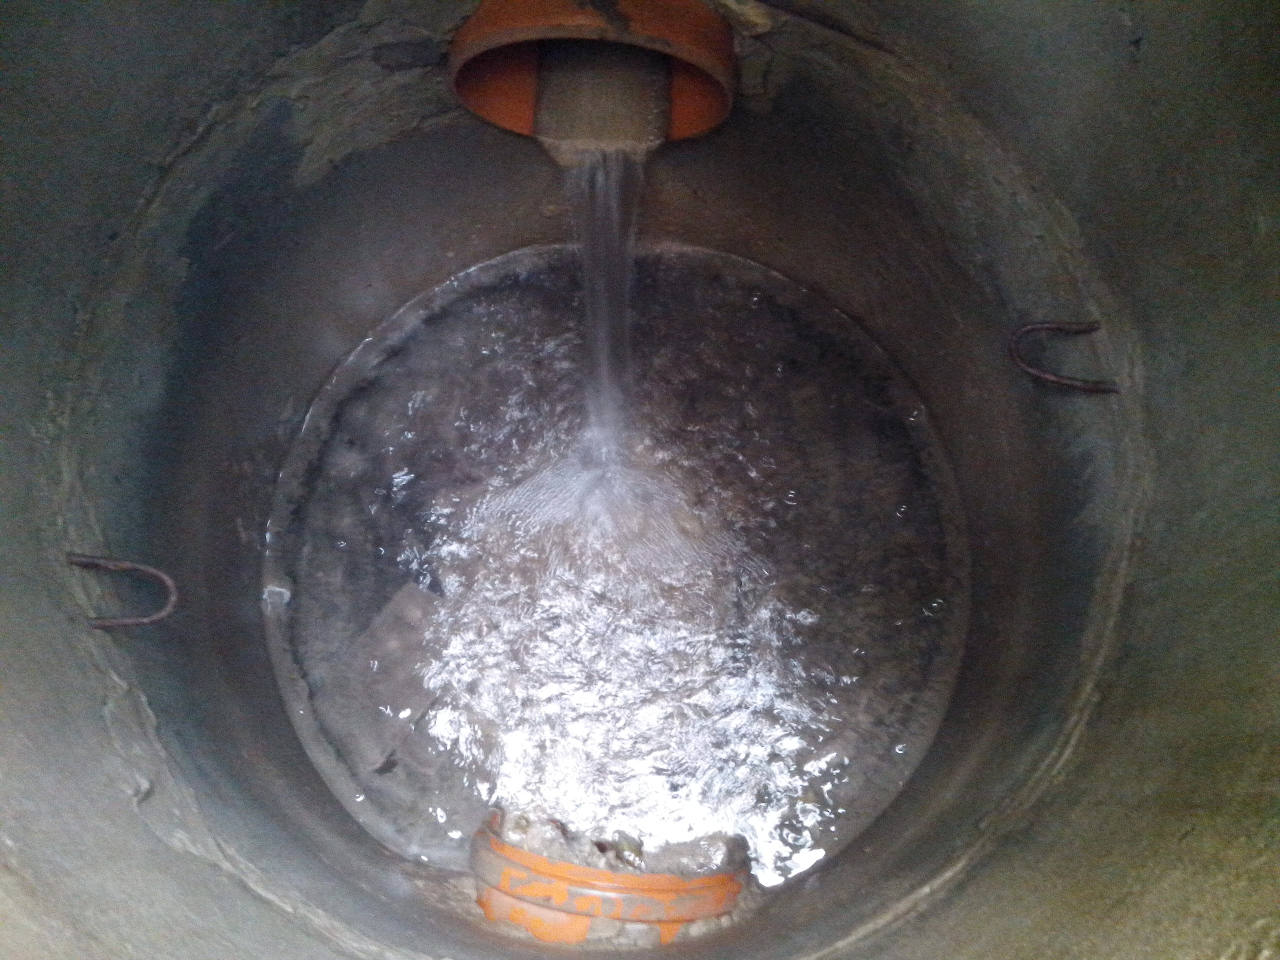
\includegraphics[width=0.85\linewidth]{chast-colebanie-osnov/borichev-tok/s_borichev-IMG_20131013_150512.jpg}

\textit{Боричев поток течет по трубам, 2013.}
\end{center}

Да, он существует по сей день, взятый в дренажную систему, именно ниже места, где стояли идолы Владимира. По склону, откуда сочился ручей, можно пройти, начав спуск с дороги на террасе под верхней площадкой фуникулера – чуть западнее тяговой подстанции, сразу за остатками древнего вала. Там на склоне будут видны остатки старой дренажки и новой, действующей. Вода шумит будь здоров – не ошибетесь!

По довольно запущенной местности, где всюду валяется мусор вперемежку со старинными кирпичами и торчат дренажные смотровые колодцы, сходит тропка к улице Боричев Ток, её концу, точнее пустырю между нею и фуникулером. Там есть примечательный розовый, о двух этажах, кирпичный дом с табличкой «Боричев Ток 4» – на разных картах его обозначают то номером 1, то вообще никак. Ниже его, на северо-восток, площадка с люком. Под этим люком вниз идет глубокий колодец, соединенный с двухкилометровым подольским коллектором Кинг Спелео – туда же впадает и труба от Боричева потока.

\begin{center}
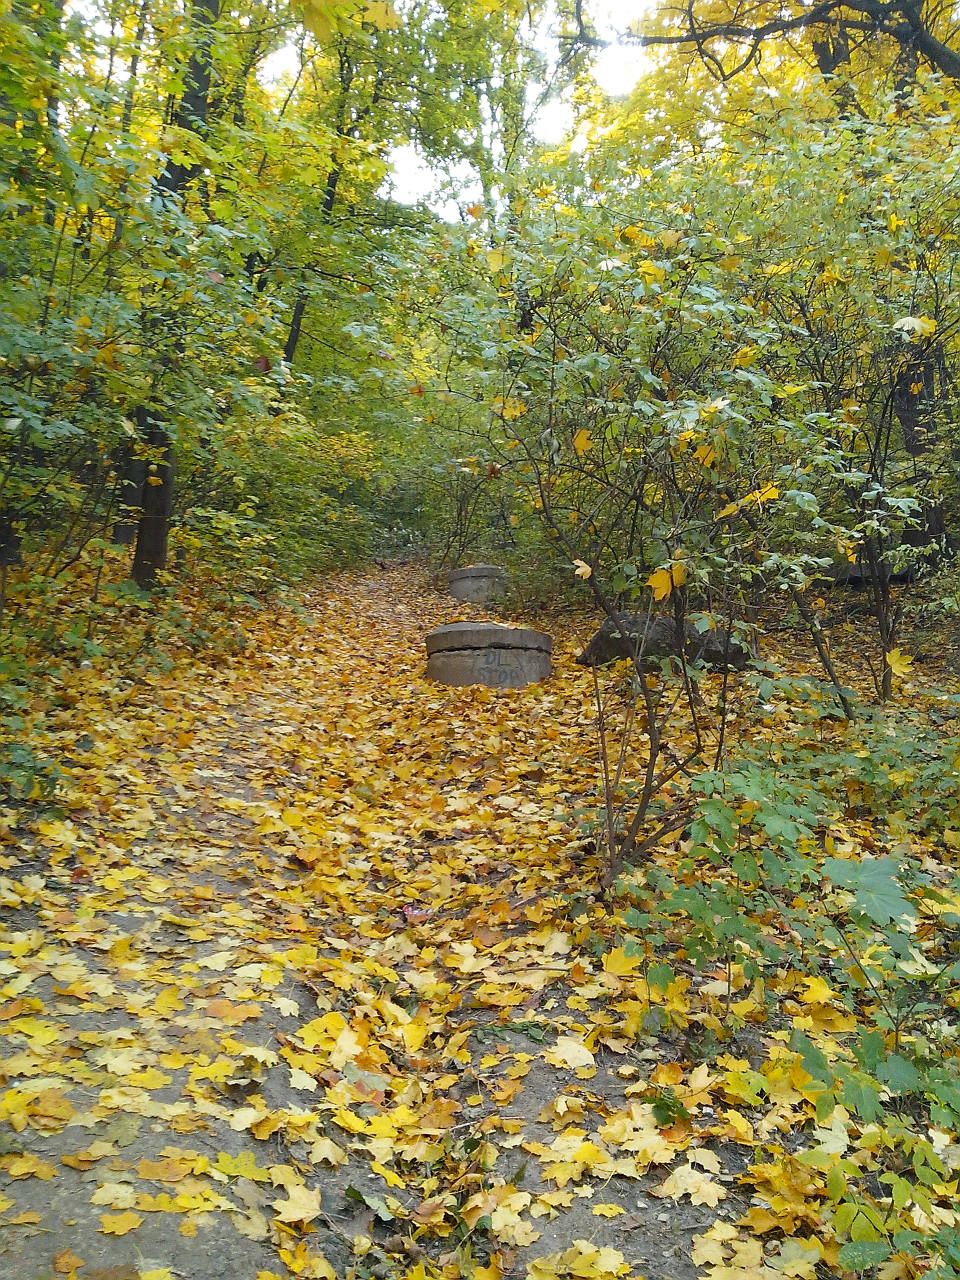
\includegraphics[width=0.70\linewidth]{chast-colebanie-osnov/borichev-tok/s_borichev-IMG_20131013_150232.jpg}

\textit{Место бывшего русла Боричева потока, 2013.}
\end{center}

Современная улица Боричев Ток известна по крайней мере с середины 19-го века. Названа по местности, слывущей так еще ранее. От протекавшего потока, окрестности стали именоваться Боричевым Током. В книге «Киев теперь и прежде» за 1888 год Захарченко описывает Боричев Ток как некое место (обращенное на восток) под крутым оврагом.

Максимович в очерке «Паны Ходыки» из  дореволюционного альманаха «Киевская старина» упоминает, что Иван Кобызевич примерно в первой половине 16 века, разбогатев, купил себе дом на Боричевом Току, как следует из земельных документов.

Нынешний Боричев Ток – довольно ровная улица, идущая под самой горой, террасой выше нижней улицы, Сагайдачного. На одной карте 1900 года Боричев Ток занимает также и современную улицу Боричев спуск, а на карте 1901 года, и других позднейших дореволюционных – теперешний Боричев спуск обозначен как Боричев извоз/взвоз.

Вот картинка. Я отсканировал ее из книги 1982 года «Киев: исторический обзор», где подпись гласит – «Гравюра 18 века».

\begin{center}
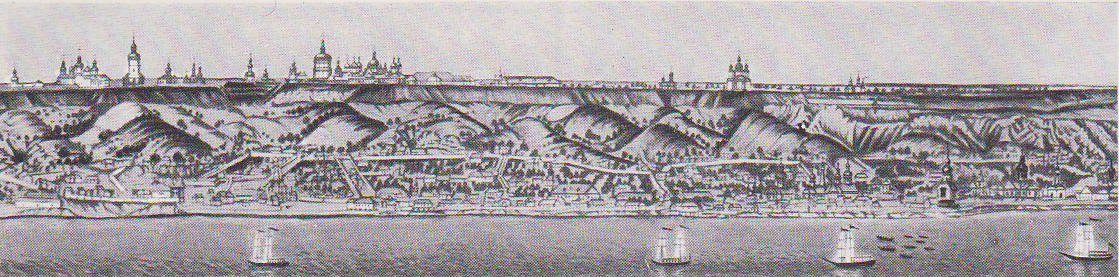
\includegraphics[width=\linewidth]{chast-colebanie-osnov/borichev-tok/18-vek-bor.jpg}
\end{center}

Не буду касаться точности изображенного, об этом судить уже трудно. Но Боричев Ток заметен здесь отчетливо – светлая дорога поперек склона горы, на высоте его середины.

Бросается в глаза вызванная оборонными соображениями обособленность нижнего города от верхнего. Никаких заездов туда по видимой части восточной стороны Старокиевского холма. Заезды, однако оборудованы снизу, на Боричев Ток, в левой половине гравюры. Там же хорошо показаны остатки «буерака». Церкви слева от него – Михайловский монастырь, справа – София, а после перерыва, еще правее – трехкупольная Андреевская.

Ровная кромка горы – следы крепостного укрепления. Конечно, врез\'авшийся в холм овраг Боричев с дорогой нарушал неприступность верхнего города и был в конце концов засыпан. А вал, показанный слева, ограждая Михайловский монастырь от края, ныне, когда мы прогуливаемся по Владимирской горке к фуникулеру, возвышается слева крутой травянистой горкой.

Художник Василий Иванович Штернберг в 1837 году написал картину «Вид на Подол»:

\begin{center}
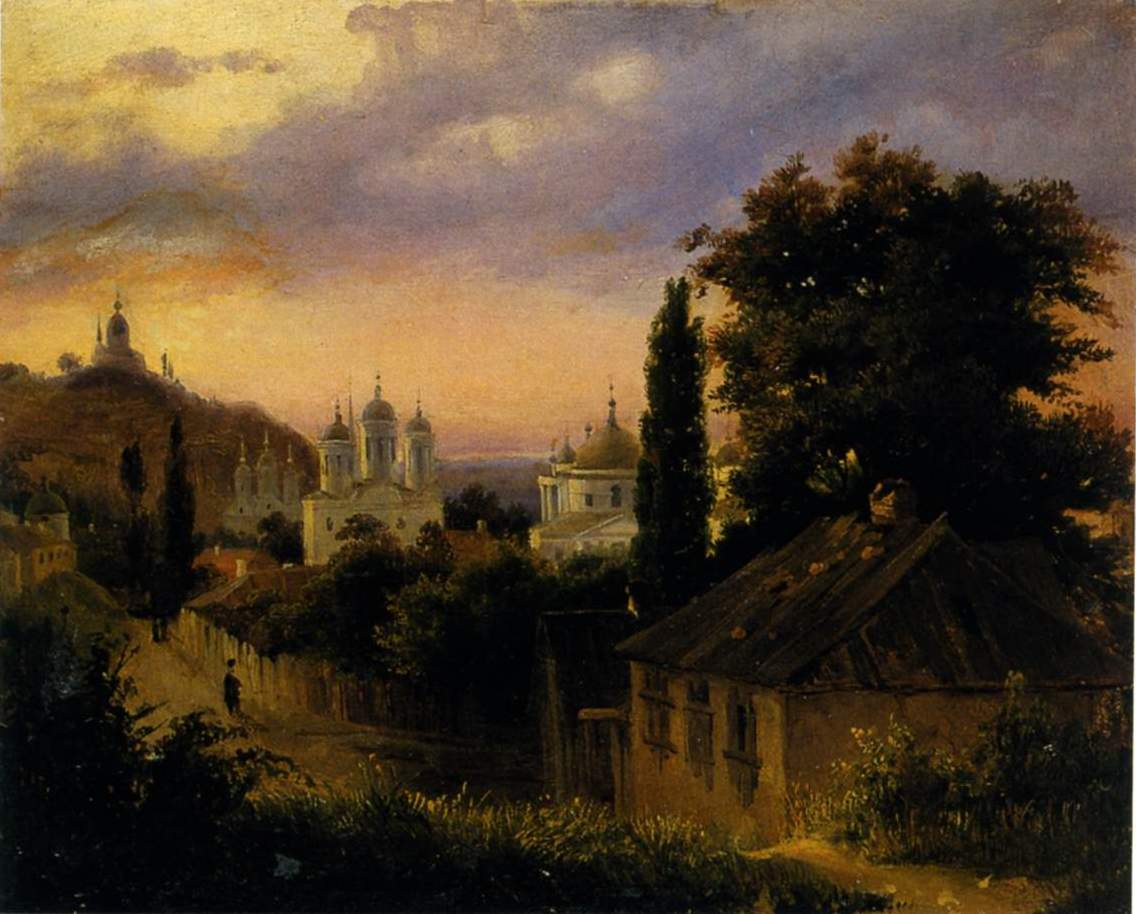
\includegraphics[width=\linewidth]{chast-colebanie-osnov/borichev-tok/st-1837.jpg}
\end{center}

Это зарисовано примерно со следующего ракурса – смотрим на север, находясь на современной улице Боричев ток в месте, где по правую руку, внизу, подходит Игоревская улица.

Две белые церкви посередке: сначала идет Покрова, а правее от нее Николы Доброго. Позади, на крутой горе Щекавице маячит церковь Всех святых.

Думаю, Боричевым Током сначала называлась местность, непосредственно примыкавшая к ручью, потоку Боричеву. Неясно, в какую сторону он протекал, равно и насколько улица Боричев Ток вышла за пределы одноименного урочища.

Еще недавно, до 21 века, улица была застроена старинными домами об одном, двух этажах – совсем немножко сохранилось их по 2015 год ближе к Андреевскому спуску. А за четырехэтажным кирпичным домом номер 8, под горой Уздыхальницей с Домом Ричарда – пепелище частной усадьбы. Нынче Боричев Ток стал «элитным», здесь возведены дорогие терема, но чем бы его ни застроили, хоть высотками, или бетоном замостили, всё равно улица будет узнаваемой на веки вечные.

На террасе выше, под пригорком с идолами, покрывая склон, находился в давнее время сад Кучинского, слывущий местом сборищ ведьм и упырей. О нем именно в таком ключе в 17 веке говорит опись владений доминиканского монастыря, да и Михаил Загоскин в романе «Аскольдова могила», вышедшем в 1833 году, упоминает Кучинскую гору и шабаши на оной. Прямо на этом пустыре с давней открытки, за фуникулером, ниже и правее, простираясь под Андреевскую церковь:

\begin{center}
\includegraphics[width=\linewidth]{chast-colebanie-osnov/borichev-tok/\myimgprefix fun05.jpg}
\end{center}

Самым же ближайшим окрестностям, по одну или другую сторону фуникулера – споры идут – краеведы отводят роль урочища Чертово беремище, связанного с низвержением поблизости некоего идола. Чертово – ибо поганских богов христиане величали чертями, бесами, змеями. Беремище – там, где его, черта, тащили. Беремя значит «ноша», не только как просто груз, но и то, что тащат или волочат.

Даты, принятые наукой, в годах от сотворения мира. 6488 – начало княжения Владимира, он ставит на холме кумиров. 6496 – крещение, низвержение идолов. Всего восемь лет разницы. А до того, как Владимир расположил свой пантеон над Боричевым, где и каким богам поклонялись киевляне, местные? Тем ли богам, что владимировы? Перун стоял на каком-то холме еще до Владимира – дед его, князь Игорь, водил туда языческую часть своей дружины для клятвы, а христиан-варягов с той же целью – к собору святого Ильи. Ранее сего, Вещий Олег с воинством клянется Перуном и скотьим богом Волосом.

Любопытно – в Повести временных лет, при Владимире, до принятия им христианства, некий Варяг, пришедший от Греков, исповедует христианство уже тайно.

После крещения Киева, Владимир ставит Васильевскую церковь на месте идолов Перуна, Хорса, Дажьбога, Стрибога, Семаргла, Мокоши. Меняется ли что-либо для поклонников Волоса\footnote{Общее житие Владимира говорит однако: «а Волоса идола, егоже именовахоу скотиа бога, повеле в Почаиноу рекоу вврещи». Кстати только в списках жития Владимира крещение происходит в Почайне, а не Днепре.} и других, неупомянутых богов, а также природных урочищ?

Владимир привозит византийских попов, напоказ при них сбрасывает установленные им же идолы, созывает на утро следующего дня народ к реке – бедных, богатых, рабов, нищих – и христианские священники их крестят.
 
Отношений Владимира с религией мы будем касаться в книге по мере надобности. Современная его оценка слишком прямолинейна и основана на личной вере. Для православных он свят, неоязычники его не любят. Однако размышления над поступками княгини Ольги да Владимира могут привести к иным выводам, нежели принято.

А знаете, как умер Красно Солнышко? Заболел тяжело и скончался 15 июля, на Берестовом, где был его княжий двор – около Лавры, а не в центре Киева, как нам говорят ученые. Для осмысленного прочтения надобно «и» после глаголов понимать как «его»:

\begin{quotation}
Умре же Володимир, князь великый, на Бересетовем, и потаиша и, бе бо Святополк в Кыеве. И нощью же межи клетми проимавше помост, в ковьре опрятавши, и ужи свесиша и на землю, и взложивша и на сани, и везоша, и поставиша и в святей Богородицы в церкви, юже бе сам создал. Се же увидевше людье, и снодошася бещисла и плакашася по нем [...]
\end{quotation}

Что означает:

\begin{quotation}
Умер же Володимир, князь великий, на Берестовом, и потаили его, потому что в Киеве был Святополк. 

Ночью же, между клетьми сделав проем в помосте, спрятав в покрывале, на веревке (ужи) свесили Владимира на землю, и положив его на сани, отвезли и поставили его в церкви святой Богородицы, которую он сам создал.

Это увидели люди и сбежались в бесчисленном количестве, и плакали по нем.
\end{quotation}

Разберемся!

Что значит «потаили» применительно к покойнику? Тело Владимира выставляют потом в церкви на всеобщее обозрение. Значит, речь не идет о сокрытии тела из каких-то соображений, связанных со Святополком.

У Сахарова во втором томе «Сказаний русского народа» я вычитал слово «опрятывать», означавшее одевание покойных в саваны и рубахи. Поскольку «таить» по смыслу подобно к «прятать», предполагаю «потаили» значит переодевание перед похоронным обрядом.

%В летописях слово «потаить», «спрятать» в отношении к мертвецу означает некое вероятно обрядное действие, совершаемое перед перевозкой покойного. Возможно, корень «таить» раскрывается через современное английское «tie» – «связывать», «заматывать». Вот же рядом – «опрятавши в ковре» – замотав в покрывало. Прятать, таить, потаить – одного поля ягоды. Потаивание же могло быть обычаем связывания покойника, отголоском опасений, что мертвый способен восстать и напасть на окружающих.

Поскольку в Киеве тогда пребывал сын Владимира, Святополк, он и «потаил» тело отца своего. На миниатюре Сильвестровского списка Сказания о Борисе и Глебе изображены два человека, опускающие в сани тело, завернутое в покрывало, и подпись сверху – «святополк потаи смерть отца своего»\footnote{Эту тему подробнее исследовал Д. Н. Анучин в работе 1890 года «Сани, ладья, кони как принадлежности похоронного обряда».}. 

Даже летом, согласно обряду, мертвеца до гроба перевозили на санях. Владимир Мономах в поучении говорит про склон лет своих – «седя на санех». Становится ясной и поговорка – не в свои сани не садись. То же относится к смутно известному фольклористам давнему преданию, ходившему кое-где по Украине, что в селах жители спускали своих престарелых родителей на санках в овраг, чтобы даром не кормить. Может и спускали, да только это были обычные для того времени похороны мертвых.

Но вот способ выноса тела Владимира Красно Солнышка из помещения кажется странным. Разбирают часть дома. Труп спускают через проем наружу, где кладут в сани и везут в церковь.

Царя Бориса Годунова считали чародеем, и по обычаю обхождения с такими людьми, останки его вынесли из Архангельского собора через пролом в стене. Также, мертвых колдунов выносили не через дверь, а через окно.

Так вот о Чертовом беремище! Полагаю, гора с ним издавна слыла священным местом. Кстати ее пронизывали пещеры. А на склоне, должно быть, было место подношений даров божествам. Такие места в старину находились по берегам многих рек. Беремя – ноша. И христиане назвали место сие – Чертово беремище, подношение чертям, божествам поганским. От противных христианам здешних празднеств и пошла слава о шабашах в саду Кучинского, позже соседствовавшего с «беремищем».

Некоторые источники именуют Чертовым беремищем дорогу «с горы» ниже Михайловского монастыря, а ею мог быть только Боричев увоз. Там больше просто негде спускаться, разве вдоль Боричева потока, да еще западнее, на склоне Владимирской горки, справа от Кокоревской беседки лестница в крутой лощине вниз идет – уклон круче Боричева. Вдоль лестницы проходит дренажка, тоже соединенная с Кинг Спелео.

В Синопсисе\cite{sinopsis} сказано:

\begin{quotation}
Идола (не уточняется, какого) егда влекоша вернии с горы утопити в Днепр, биюще его нещадно [...] и оттуда дорогу ту с горы нижае монастыря Золотоверхно-Михайловского нарекоша древле Чортово Беремище, си есть, тяжко черту.
\end{quotation}

Софонович в «Кройнике» пишет уже с подробной привязкой к местности. Он рассказывает о низвержении кумира, причем не говорит, что это Перун. Просто «один балван»:

\begin{quotation}
Повесть теж есть старая тая, же гды едного балвана волокли з горы утопити в Непр и били по череву, бес в нем кричал, лементуючи. Оттол тую з горы дорогу нижче монастыря Михайловского здавна назвали Чортово Беремище, то есть тяжкость чорту, бо слово славенское «бремя» значит «тяжкость». И гды того балвана утопили, плынул вниз, а неверныи, идучи берегом, плакали и звали, мовячи: Выдыбаи наш Гсдрю Бже, выдыбаи. А тои балван выдыбал аж там на берег, где теперь монастырь Выдубецкий, и названо тое местьце тым урочищем от выдыбаня Выдабича албо Выдубичи.
\end{quotation}

А также, говоря о создании Михайловского монастыря:

\begin{quotation}
Митрополит Михаил, посадивши ченцов на горе, не далеко от того беремища чортова, на свое имя церковь Святаго Архангела Михаила збудовал, иже як з неба святый Михаиль чорта зкинул, так тут он же погнал згоры чорта вболване збивати.
\end{quotation}

%И дополняет на обороте листа 31 о приказе Владимира:

%\begin{quotation}
%Перуна балвана, к хвосту конскому привязавши, казал у Днепр волочи и утопити, а там црковь Свтго Спаса каменную поставил. Наипервеи в свое имя казал црквь Свтго Василия поставити на горе[...]
%\end{quotation}

%Спасская церковь на Подоле стояла до пожара 1811 года, как полагают, на месте нынешнего дома по адресу Спасская, 31. Место ли это древней Спасской церкви, неясно. От церкви святого Василия, верхней площадки фуникулера – до указанного адреса – более километра на север, причем удивительно по прямой линии!

%Но если первоначальная церковь Спаса была именно там, возникает вопрос. Ежели Софонович передает истинное положение места о ввержении в воду идола Перуна, то зачем его тащили так далеко? Ведь река ближе на восток, у Почтовой площади. 

Можно ли по письменным свидетельствам проследить связь между Чертовым беремищем и другими урочищами? 

Выдержка из документа «Опись актов и недвижимых имуществ Златоверхо-Михайловского монастыря», за 1646 год. Она дает нам дополнительные ориентиры сразу по двум местностям, саду Кучинского и Чертову беремищу. Речь идет об одном пляце, земельном участке, принадлежащем монастырю:

\begin{quotation}
Пляц, лежачий под горою и валом, вышовши з манастыря калиткою, по левом боце звозу Михайловского, у урочища, прозываемого Чортова Беремища. Граница того грунту: почавши от горы уз дорогу куды ходят з места до манастыря Михаловского, мимо тот двор, аж до саду Кучинского из другои стороны валом аж до тыну священника Рождественского под гору.
\end{quotation}

Разбирать старинные грамоты – лучшее средство от сна. Лежишь полночи и в голове у тебя крутятся, крутятся трактовки. Всё настойчивей понимаешь, что надо ехать на местность, лазать, смотреть всё своими глазами, щупать ложноножками, прикидывать.

Во время составления всех этих грамот, слова имели определенные значения, и описания давались с точностью достаточной, чтобы соответствовать местности и служить доказательствами. Не должно было возникать вопроса – а какой вал? А какой дорогой ходят к монастырю «з места»? «Место» – значит «Подол»? Первый упомянутый вал – тот же, что и второй?

Первый вал – думаю, это горизонтальный вал по вершине, краю холма. И второй вал до сих пор существует, я о нем говорил – спускается вдоль северо-западной стороны рельсов фуникулера. 

А внизу у нас что? Церковь Рождества. Что сказано в земельном акте? «До тыну священника Рождественского под гору» – до тына священника Рождественской церкви, которая под горой, на нынешней Почтовой площади (прежде храм сей стоял ближе ко склону, чем ныне). Значит, речь идет именно о вертикальном вале рядом с фуникулером. Вал нисходил до тына священника.

Я бы трактовал всё так, по современным ориентирам – пляц, как если идти от фуникулера по дороге на террасе под верхней площадкой фуникулера, в сторону Андреевской церкви. Пляц скоро упирался в сад Кучинского, что залезал сюда по склону.

В Универсале гетмана Мазепы в подтверждение владений Михайловского монастыря, упомянут также «пляц, под горою лежачии урочища, прозиваемого Чортово Беремища».

Хорошо, а что за Михайловский звоз? Это всё та же дорога по линии нынешнего фуникулера – позже, в главе про Почайну мы познакомимся с документальным подтверждением этого, пока же примем на веру. Далее, написано: 

\begin{quotation}
люди, под горою и на горе живующие, почав от церкви Воздвиженской даже от фортки Острожской в ров Боричов по ввоз Рождественской, куницу давали церкви вышепомянутые.
\end{quotation}

Поскольку, как я понимаю, старый Боричев увоз это Михайловский звоз, то ров Боричов – это не Боричев увоз, однако нечто соседнее. Рвом, ровчаком в документах того времени порой называли рукотворную канаву для отвода ручья. 

А Рождественской ввоз – где? Около Рождественской церкви. Возможно, прообраз Владимирского спуска. От рва Боричева граница имения шла по ввоз Рождественской.

Воздвиженская церковь здесь не нонешняя под Замковой горой. На плане Ушакова 1695 года видно, что Воздвиженская церковь стояла наверху Старокиевской горы, в окрестностях появившейся позже Андреевской церкви. Где была фортка Острожская – сведений нет. Профессор Петров в угоду своему видению топографии располагал её около Чёрной грязи (сейчас это удолье, ограниченное Замковой горой, Андреевским спуском, улицами Боричев Ток и Флоровской).

Возражу. На том же плане Ушакова, непосредственно выше церкви Воздвижения, показан комплекс Приказной палаты из нескольких зданий. А в приказной палате кроме прочего есть тюрьма. Значит острог. Далеко ходить поэтому не надо. «От церкви Воздвиженской», и уточнение – «даже от фортки Острожской».

В грамоте описываются места строго сверху вниз: острог, Воздвиженская церковь, Боричев ров, Рождественской ввоз.

Острогом раньше называли, кроме прочего, по Далю, «укрепленное тыном заселение». Деревянную ограду Подола тоже называли острогом. За год 1654 о ней сказано: «было острогу сажень с 300 а по тому острогу было 6 башень да двои ворот проезжие»\cite[том X, стр. 387]{akty}. Но церковь Воздвиженская была наверху, на Уздыхальнице или ближе к Андреевской, поэтому и фортка Острожская относится к той же местности.

Кстати, в «Обозрении Старого Киева» у Максимовича есть примечание: 

\begin{quotation}
Некоторые киево-подольские старожилы помнят, что в 1810 году, когда для построения нынешней каменной церкви Рождественской разбирали прежнюю деревянную, построенную 1564 года, то в ее основании найдено было надписание, что она поставлена была на увозе Боричевом. 
\end{quotation}

Этому сообщению ученые, считающие увозом Боричевым Андреевский спуск, просто не верят. Мол, обманулся доверчивый Максимович. По простоте. Кажется, если найдут кем-то в старину вбитый на Боричевом спуске столб с названием, то ученые отвергнут и сей довод. Ибо не вписывается в их «убедительно доказанное».

Сад Кучинского (Кучовского) упоминается в давних земельных бумагах, а проповедник доминиканского монастыря Петр Развидовский, в записках 1630-60 годов, доносит молву про этот сад: «где ведьмы слетались».

Среди краеведов уже три века идут споры, где же находился этот зловещий сад. Споры сводятся, грубо говоря, к выбору между двумя вариантами – по одну сторону от фуникулера или по другую. Некоторые полагают бывший сад вовсе посередке. Между тем архивные источники дают довольно точный ответ. Изучение вопроса заодно развеивает краеведческую байку о местности под названием Сколники, которую исследователи киевской старины голословно переименовали в Сокольники и связали с соколиной охотой. Но давайте по порядку.

В 17 веке был такой Мацей Кучинский. Он и его семья владели землей в местности Сколники, в окрестностях Боричева.

В «Грамоте Царей Иоанна и Петра Алексеевичей, подтверждающей Киево-Братскому монастырю права на принадлежащие этому монастырю земли и угодия. 1694. Января 11»\cite{sbornikmat}, читаем – что ни слово, то золото:

\begin{quotation}
В купчей инокини Парасковии Кучинской, 1621 году: что подала она в Братский монастырь двор свой Кучинской, на котором дворе семнадцать человек обретается, и подати ей з земли платит. А тот двор ея с иными местами лежит в Киеве под горою в Скольниках, против церкви Рождества Христова. А взяла она за тот свой двор и с местами тысячи коп денег литовских.
\end{quotation}

И ниже в тексте:

\begin{quotation}
Двор Катерины Кучинской, купленный за тысячу коп литовских под горою городовою, по улице, лежащей от церкви Рождества Христова к площади торговой.
\end{quotation}

Итак, более-менее прояснилось. Кучинская владела двором и иными местами – а они находились под горою рядом с церковью Рождества Христова, и оттуда по улице в сторону торга, то есть к нынешней Контрактовой площади, где ранее был торг (не Житний). Улица эта, по сведениям Похилевича\cite{pohilmon}, тогда, до знаменитого пожара 1811 года, называлась Гнилой по своему водянистому состоянию, и шла наискось от церкви Рождества, мимо Николы Доброго да к Братскому монастырю – стало быть и торгу.

Что до земель Кучинской, речь идет о начале современных улиц Боричев Спуск и Боричев Ток. И оттуда пространство в сторону Контрактовой площади. В своей книге «Киево-Братский училищный монастырь» Мухин трактует «17 куничников» как «17 оброчных дворов». А можно и – на земле Кучинской обитало 17 семей, которые платили землевладелице налог, куницу.

Какие «иные места» были у Кучинской? Сохранилась «Продажная запись инокини Параскевии Кучинской Богоявленному монастырю на свой пляц около Рождественской церкви»\cite{muhin01}, от 5 июля 1621 года. Я начал переписывать её сюда целиком, однако на четвертой странице бросил, не в силах более переносить канцелярский язык того времени. Ограничусь пересказом и приведу наиболее важное.

Продажная запись составлена инокиней Киево-Печер\-ского монастыря Катериной, в иночестве Парасковьей, вдовой Севастиана Фронцевича. Катерина была дочерью Мацея Кучинского. И вот она продает 

\begin{quotation}
\textbf{добра мои власные дедичные в месте короля его милости Киеве лежачие, то ест пляц в Сколникох под горою противко цер\-кви Рожества Христова}, збудованем также и з семнадцатма куничниками на нем оселыми будучи волный никуничный никому ни чим не ценный и не заведенный, а ни жадными долгами зысками презысками не обтяжоный, \textbf{такъже з садом огородом} и огорожою платою куниц и зо всим на все ?косе в собе вдолж и вширь ростегает зо всими пожитками и принадлежностями \end{quotation}

Сад упомянут и в другом месте документа:

\begin{quotation}
А по заплаченю того закладу и по нагороженю шкод вышейменованых пред сесь лист вечистое продажи запись мой во всих своих артыкулах пунктах кондыциях и клявзулах у кождого суду, права и на пождом местцу при зуполной и досконалной моцы захован и держан быти мает вечными часы и о вшем еслибы кто колвек в держанъю и вечистом уживаню тых добр \textbf{кгрунту пляцу и саду} вышъменованого и пожитков
\end{quotation}

Есть также волшебная «Выпись из книг киевской ратуши, с прописанием меры монастырской земли в Киеве на Подоле»\cite{muhin01} от 26 мая 1693 года. В ней рассказывается, как различные официальные лица являются на место измерять и описывать. И вот:

\begin{quotation}
напрод пришовши до пляцу прозываемого Кучинского, купленого за тисячу коп у Катерины Кучинское, лежачого под горою замковою, на улицы идучой от церкви Рождественское на рынок, з кождое стороны мералы оный; а так той пляц, з одное стороны через улочку якая взалася з пробитое улицы на гору, против пляцов Рождественских, есть аршинов Московских двесте и десет до горы, з другое стороны от пляцу пана Григория Карповича бывшого полковника Киевского, не до самое горы (бо за пляцом пана Карповичовым еще даней той пляц зайшол) аршинов сто осмънадцат и четверт, того теж зайстя долиной вдолж аршинов сто осмдесят пят и три четверти, а оттул до горы уз пляц отца Илии Священника Добро-Николского аршинов девятнадцать и шест, в тылу от горы аршинов двести сорок и три, а на улицу уз ворота аршинов двесте и шестдесят.
\end{quotation}

Вникнем. Первое, что бросается в глаза – указание на замковую гору. Это сейчас Замковой считают одну только Киселёвку в теперешнем её состоянии. Замок Киевский, однако, покрывал и окрестности, включая отрог Уздыхальницу.

Начинаем вычисления. 1 аршин – 0,71 метра. Также я думаю, что опорой нам послужит план Ушакова, ибо хоть пожары, хоть год 1695, а всё же относительное положение объектов на местности думаю, сохранялось. Я не буду сейчас говорить про стороны света, удобнее лево-право, касательно картинки. План зарисован, как если стоять лицом к холму.

%Глядя на следующий кусок карты, проще понимать цитаты.

\begin{center}
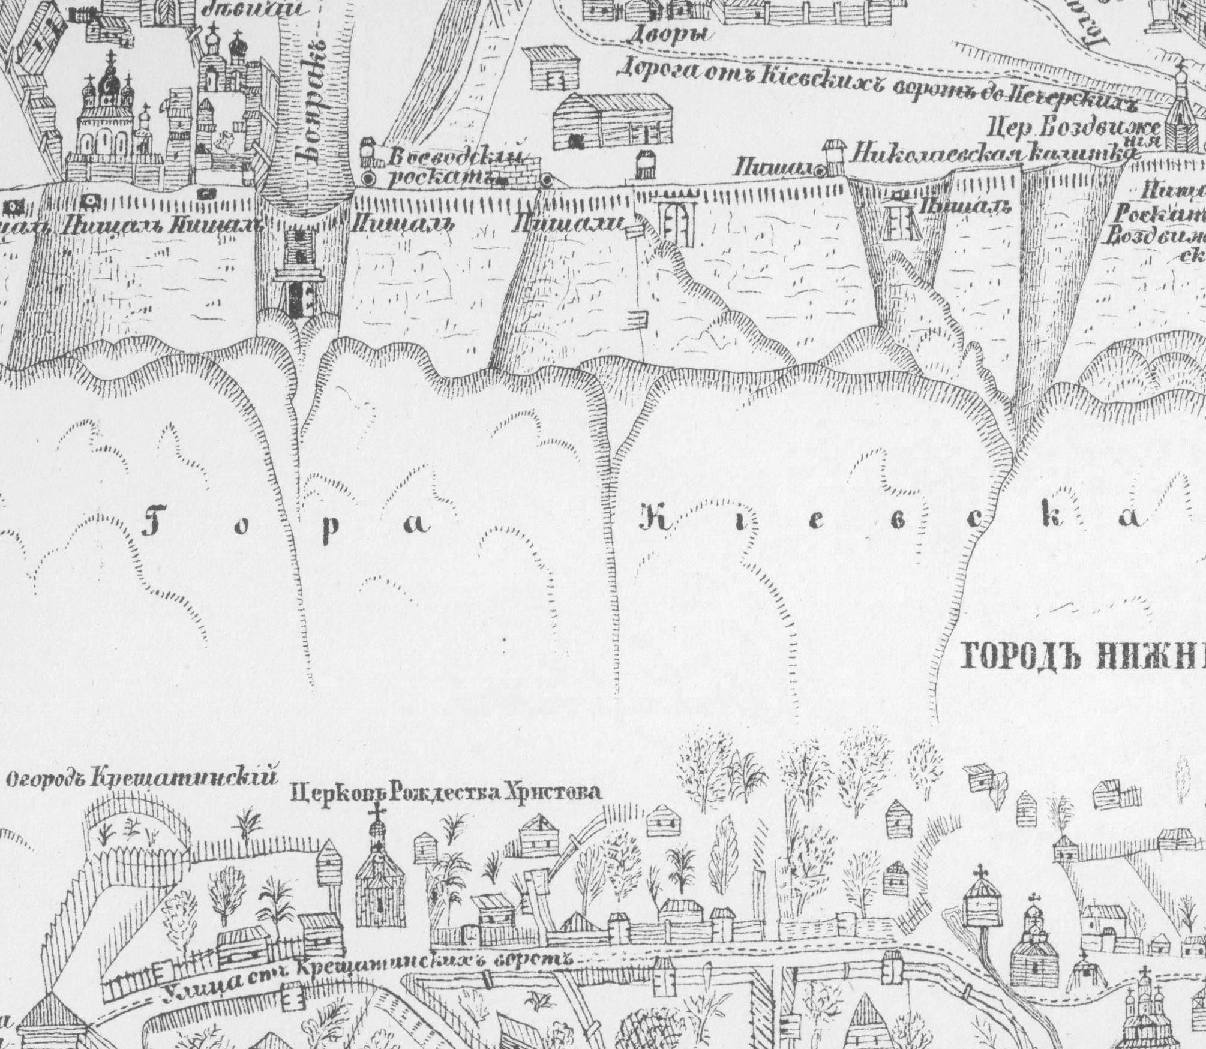
\includegraphics[width=\linewidth]{chast-colebanie-osnov/borichev-tok/1695-kuch.jpg}
\end{center}

Слева от церкви Рождества, возможно, огород ее священника. Справа начинается пляц Кучинского. В правой части карты, ниже надписи «Город нижний Подол», на одном уровне с церковью Рождества – две церкви, Покровы и Николы Доброго, которая «стояла на потоке», и оттуда ручей протекал дальше вдоль переулка. Не Боричев ли это поток туда достигал – спустившись со склона и повернув под ним, направлялся к Николе Доброму, а там снова поворачивал, уже к берегу Почайны (так в то время именовался на протяжении Подола ближайший к правому берегу рукав Днепра)? Почайну мы обсудим в отдельной главе.
 
\begin{quotation}
а так той пляц, з одное стороны через улочку якая взалася з пробитое улицы на гору, против пляцов Рождественских, есть аршинов Московских двесте и десет до горы, 
\end{quotation}

Возле Рождественской церкви на гору восходит улица. Правая её сторона и есть юго-западная граница пляца Кучинского. Обмер таков: 0,71*210=149,1 метра. Это примерное современное расстояние между началами улиц Сагайдачного и Боричева Тока, еще залезая на склон. Границей пляца можно приблизительно считать четную сторону улицы Боричев спуск, от перекрестка с Сагайдачного.

Противоположную границу предлагаю понимать примерно как окрестности церкви Николы Доброго (на это есть еще одно указание относительно арендатора Лейзора, о чем будет сказано ниже), где пляц Кучинского примыкал к горе. 

Между горою и Николой Добрым была еще армянская церковь Рождества Богородицы (говоря языком документа 1622 года, «костел Орменский», «нароженя найсветшои Панны Марии»), сгоревшая в 1651 году. О прилегающих её владениях мне ничего неизвестно. В 1685 на её фундаменте возвели деревянную церковь Покрова Пресвятой Богородицы на Подоле. В 1766 или 1772 году здание оной заменили на каменное.

Более известный ориентир – Андреевская церковь на холме. Сад доходил к склону под нею. Вот так проще.

Верхняя граница земли Кучинской не постоянно шла примыкая к самой горе, но в каком-то месте отклонялась от нее имением бывшего полковника Карповича.

Сколники. Судя по всему, это местность, лежащая от Контрактовой площади до Почтовой. Что значит слово «Сколники»? Некоторые части Подола назывались по принадлежности к профессиональным цехам – например, кожевники жили на Кожемяках, гончары в Гончарах. Участок на юго-восток от Почтовой площади, вдоль набережной, в сторону нижнего памятника Владимиру (колонны Магдебургскому праву), в начале 19 века именовался «Кузнецы».

А сколники это кто?

Сементовский в «Киеве»\cite{sement01}, в разделе про улицу Александровскую (сейчас это Сагайдачного) упоминает Сколники, переиначив их в «Соколье или Сокольники», по подобию московских, и пишет, мол, тут «судя по названию содержались соколы и жили сокольники великокняжеской ловчей дружины». И вот он судит по одному только названию, а затем вдруг пускается в подробности, что князья, отправляясь охотиться на острова, спускались по Боричеву, останавливались в Сокольниках, там готовились, и затем шли к пристани тут же неподалеку.

Верить Сементовскому? Он приводит еще маршрут ведьм, которые, слетаясь на шабаш, делают вначале остановку в саду Кучинского, отдыхают там, а затем уж перелетают через Днепр к левобережной Лысой горе.

На польском и литовском языках слово «skolnik» значит «школьник».

Священник Иоанн Лукьянов в 1701 году, путешествуя, по пути в Палестину посетил Киев и оставил об этом записки\cite{sbornikmat}. Кроме прочего он сообщает:

\begin{quotation}
В Киеве на Подоле град деревянный, и грязно сильно на Подоле. А жилье в Киеве в верхнем городе и в нижнем – все в городе, а за городом нет ничего. В Киеве школьников очень много да и воруют много; попущено им от митрополита. Когда им кто понадокучит, тогда пришедши ночью да и укокошат хозяина-то; а из двора корову или овцу сволокут; нет на них суда, скаредно сильно; попущено воровать пуще московских солдат; а вечер пришел, то и пошли по избам псалмы петь, да хлеба просят; дают им всячиною и деньгами и хлебом, а иные им дают убоясь.
\end{quotation}

Да ведь это же бурсаки! Та часть Подола была наводнена учениками находящейся там же Академии, Братского училищного монастыря! Потому и местность называлась Сколники – школьники! А частью самих Сколников, примыкающей к горе, был меньший район – Боричев Ток.

На Сколниках стояла, посередке короткой улицы Покровской, церковь Николы Доброго, что прослеживается здесь по меньшей мере с 16 века, когда деревянной ея с богадельней выстроил гетман Самийло Кошка, он же Матвей Кушка. Храм сжигали, восстанавливали, разбирали, возводили заново. С 1651 по 1662 год он лежал в выгоревших руинах.

В 1651 году казаки грабили и громили Киев. Хроника, перечисляя разрушения, упоминает о сожженных Флоровском монастыре, монастыре Бернардинов и деревянной церкви Доброго Николы. Позже её отстроили, опять из дерева. Потом сгорела дотла от удара молнии. В 1705 году на развалинах поставили уже каменный храм. Колокольню при нем соорудили, вероятно, в те же годы. Через сто лет церковь разобрали, а в 1800-1807 годах опять возвели, по проекту Андрея Миленского, и в последний раз развалили в 1935-м, однако часовня уцелела по наши дни. 

Ее адрес – улица Покровская, 6, на углу. На месте самой церкви сейчас корпус лицея, ранее школы, номер 100. А вот Покровская 4 – это, как мы увидим дальше, место бывшего типографского двора доминиканцев. Напротив, на другой стороне улицы, церковь Покрова. Всё это у подножий отрогов Старокиевской горы – Андреевской горы да Уздыхальницы.

«Поток», на котором стояла церковь Николы Доброго, в научной литературе слывет как «Борисоглебский ручей», хотя это название чисто книжное. Просто увидели на плане Ушакова «переулок по нему же ручей», нарисованный от Покровы, мимо Николы Доброго и продолжающийся примерно по ходу теперешней улицы Борисоглебской, где на месте домов номер 10, 11 находился одноименный деревянный храм. И решили ученые назвать ручей «Борисоглебским».

Он вроде существует по сей день и до 2012 года протекал, по словам диггеров с сайта ACIS, в яйцевидном кирпичном коллекторе метровой высоты, наполовину замытом, а кое-где в трубах. С 2012 – вместо кирпичного коллектора проложена труба.

Сведения о ручье у Николы Доброго имеются следующие. Лаврентий Похилевич, малоизвестная книга «Монастыри и церкви Киева»\cite{pohilmon}, заметка про «Доброниколаевскую церковь». Там помещено Сказание о пленном Половчанине, который приносит клятву около церкви «святого Николы». До сих пор ломают голову, с какой из церквей Николы её соотнести. Похилевичу удалось разыскать вариант сказания с подробностью, что церковь стоит «на потоке». Он приводит текст по древней рукописи, хранящейся в Софийском соборе, где описано «Чудо святого Николы, которое сталось в месте Киеве на Добрыку».

Историю эту относят к 12 веку. Добрыком звали человека, у коего в плену был Половчанин. Добрык хотел освободить пленника, но за выкуп. С собой денег у Половчанина не оказалось.

\begin{quotation}
Теды Добрик, приведши его до церкви, которая до сего часу стоить на потоке, под горою в Киеве
\end{quotation}

Добрык предложил пленнику взять в поручители святого Николая, то бишь поклясться оным, что будучи отпущенным, Половчанин привезет за себя выкуп. Тот дал клятву и скрылся, не думая ничего привозить. Но святой Николай явился к нему трижды, причем в последний раз не келейно, а при «многолюдном обществе», и заставил отдать Добрыку выкуп стадом лошадей, еще и сверх того 10 белых коней.

Вне рукописи «от Похилевича», история эта известна в менее краеведческом варианте как «чудо святого Николая о Половчине», относящееся к посмертным чудесам Николая Мирликийского. Текст ея находим, кроме прочего, в 72 выпуске серии «Памятников древней письменности и искусства» 1888 год, в статье архимандрита Леонида (Л. А. Кавелина) «Посмертные чудеса святителя Николая, сочинение Ефрема Переяславского XI века». Вместо Добрыка там действует некий «целомудренный человек», имеющий веру великую и любовь к святому Николе. И сей человек привел Половчина для клятвы к церкви «святого Николы» – не указано, что на потоке.

Итак, сочинитель рукописи, известной Похилевичу, соотнес упомянутую в «чуде» церковь святого Николы с церковью Николы, которая стоит на потоке под горою в Киеве, по рукописи – «до сего дня».

Константин Николаевич Гупало в книге «Подол в Древнем Киеве» сообщает:

\begin{quotation}
Именно под склонами Старокиевской горы, где сейчас проходит ул. Боричев ток брал своё начало так называемый Борисоглебский ручей, обозначенный на плане Киева 1695 года. Следы этого ручья были зафиксированы при раскопках на усадьбе бывшей Покровской церкви (1766), а также в геологическом разрезе трассы строительства метро по оси ул. Борисоглебской. Именно такое направление – от Покровской церкви мимо Борисоглебской церкви к Днепру имел ручей на плане 1695 года.
\end{quotation}

Гупало пишет еще об одном ручье в тех же краях, между «Борисоглебским» и Глубочицей:

\begin{quotation}
Во время раскопок под Замковой горой (на месте строительства Житнего рынка) было зафиксировано еще одно русло еще одного ручья. От северо-западной оконечности Замковой горы он направлял своё течение на юго-восток мимо церкви Николая Притиска (1631) к Днепру. Его русло еще дважды было зафиксировано археологически между улицами Героев Триполья и на улице Волошской. Ручей должен был впадать в Днепр – Почайну в непосредственной близости от Ильинской церкви.
\end{quotation}

Героев Триполья – это нынче Спасская, а церковь Николая Притиска имеет адрес Хоревая, 5-А. На свои деньги ее в 17 веке выстроил прихожанин Пётр по прозвищу Железный Грош. Еще раньше на этом месте стоял деревянный храм во имя того же святого. Предание гласит, что некий вор, ограбив церковь, застрял в окне – был «притиснут», потому и Николы Притиска.

Был ли это самостоятельный ручей, или может Гупало рассказывает о каком-то старом русле Глубочицы? Жаль, что не приведены подробности. Как ученые датируют этот ручей – найдены ли в нем предметы, кости, и каков культурный слой над ручьем? «Прижизненная» ширина и глубина ручья? На какой глубине обнаружен? Получается слишком много длинных ручьев, параллельно текущих в сторону Почайны. Хотя может, в древности так оно и было – канавами отводили из-под гор влагу, осушая обжитую низменность.

Вернемся к Николе Доброму. Как соотносился с ним на местности сад Кучинского? Северная граница сада была между земельным участком Николы Доброго и склоном горы, вероятно залезая на сам склон.

Петр Развидовский, главный проповедник в киевском доминиканском конвенте (монастыре) святого Николая, в записках 1636-64 годов говорит о владениях монастыря. Кроме прочего это: 

\begin{quotation}
Грунт под горою Здыхальницей от замку с сей стороны подле бернардинов. На сей грунт имели мы привиллегию короля Владислава четвертаго в разсуждении воды Кошинки, или колодезя, обрубом обделанного. Оттуда вода проведена была трубами к конвенту св. Николая с немалым иждивением конвентским и владели мы тою водою и грунтем до самой корсунской войны (1648 г.).
\end{quotation}

Грунт значит – дворовое место, единица поземельного владения. Речь идет об участке под Здыхальницей, находящемся с этой стороны замка возле Бернардинов, монастыря ордена бернардинов. Он был в месте, известном как Черная грязь, у подножия Киселевки, примыкая к теперешней ограде Флоровского монастыря.

Колодец Кошинка, в итоге превративший округу в Черную Грязь, изображен даже на плане Ушакова – вот, изливается из горы посередке картинки. Здесь же, слева, уже известные вам церкви Покровы и Николы Доброго:

\begin{center}
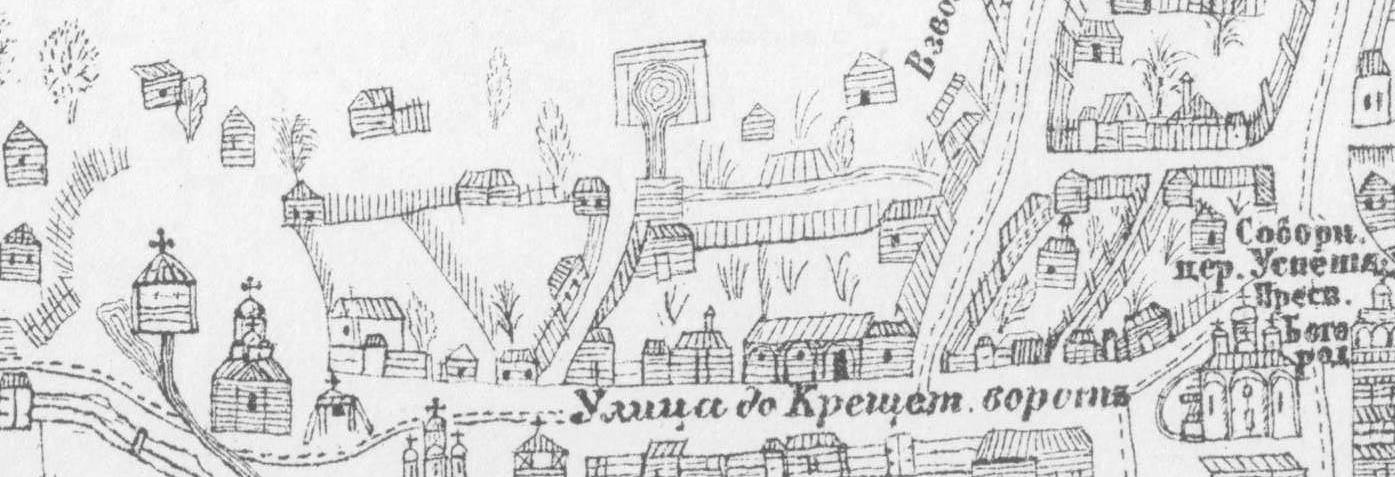
\includegraphics[width=\linewidth]{chast-colebanie-osnov/borichev-tok/s_koshinka.jpg}
\end{center}

А доминиканский каменный конвент святого Николая, постройки первой половины 17 века, находился напротив Флоровского монастыря к востоку, на другой стороне Притиско-Николаевской улицы. Здания монастыря занимали там почти весь квартал до Житнего торга, и катедра святой Софии, позже переделанная в Петропавловскую церковь, стояла на месте нынешней военной части, точно против входа во Флоровский монастырь.

В конце 16 века у доминикан были другие, деревянные кляштор с костелом, на север от Житнего рынка. После постройки каменного конвента, старый, деревянный костел перенесли куда-то «за Днепр» в имение Феодора Креницкого.

Развидовский пишет о «грунте к Днепру за бернардинами» (то есть от их монастыря в сторону Днепра – на восток либо на северо-восток, однако примыкая ли непосредственно к Бернардинам?) около грунта еврейского арендатора Лейзора, и что там был – внимание! – деревянный типографский двор между Лейзором и «садом Кучовскаго, где ведьмы слетались». 

Уточнение про арендатора Лейзора находим в «Показании игумена Феодосия Васьковскаго о положении киевских мещан до Богдана Хмельницкого», за год 1699, где упомянуто, что Лейзар жил возле церкви «Святого Николы Доброго».

Итак, Лейзор жил возле Николы Доброго. Между Лейзором и садом Кучинского был типографский двор доминиканцев. Это где? У Закревского в «Описании Киева» читаем\cite{zakr01}:

\begin{quotation}
Каменный дом и аптекарский магазин находятся на Подоле, у подошвы этого горнаго уступа\footnote{Речь идет об уступе, на коем был по мнению Закревского сад Кучинского.}, против дома Управы Ремесленных Цехов, где в 17-м веке был Типографский двор Доминиканов.
\end{quotation}

Об этой же аптеке, основанной в 1770 году, Закревский пишет: 

\begin{quotation}
В Киеве, на Подоле, возле церкви Покрова, находится большое казенное заведение сего рода.
\end{quotation}

Современный адрес дома Управы Ремесленных Цехов – улица Покровская, 4. Там стоит белый, трехэтажный «старый контрактовый дом» – первоначально именно этого назначения, а после восстановления от пожара, с 1819 по 1835 год – Управа ремесленных цехов. Потом, с 1872 года, генерал-губернатор Васильчиков открыл там Подольскую женскую гимназию. В 1879 году к контрактовому дому был надстроен второй этаж (до пожара 1811 года второй этаж был, деревянный, да сгорел), в 1901 – третий. 

После революции, в здании гимназии поместилась трудовая школа номер 19. Когда церковь Николы Доброго снесли, на ея месте к школе сделали пристройку, левое крыло – здание по адресу Покровская, 8. Позже школа получила новый номер, сотый, а с возвращением капиталистического общественного строя её переименовали в лицей. Бытность этой школы в 1930-е годы описана Александром Копыленко в повести на украинском языке «Дуже добре» и её продолжении «Десятикласники».

\begin{center}
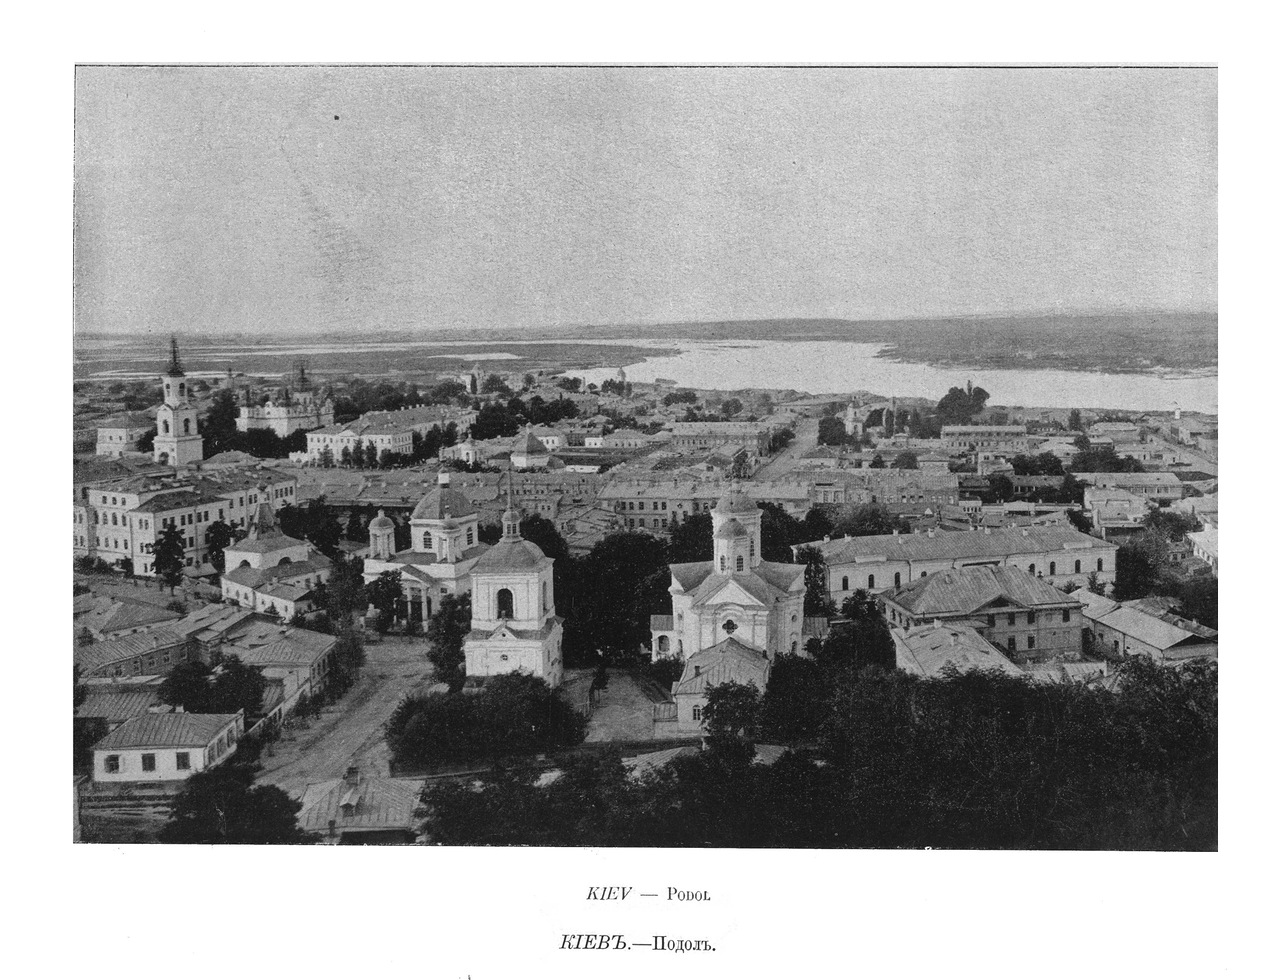
\includegraphics[width=\linewidth]{chast-colebanie-osnov/borichev-tok/podol-panorama.jpg}
\end{center}

На ладном дореволюционном снимке, сделанном, кажется, с паперти Андреевской церкви, описываемый мною район расстилается как на ладони. Улица Боричев ток лежит непосредственно внизу кадра, скрытая зеленью. Крыша в левой нижней части, куда подходит вертикально переулок – это дом по адресу Боричев ток, 23/2. Позже я покажу его на фотографии 21 века. Посередине – храм Покрова и колокольня при нем. Левее и глубже соседствуют церковь Николы Доброго со своей низенькой колокольней.

Перед ними, поперек кадра – улица Покровская. Сойдем туда.

Если встать сегодня на Покровской лицом к одноэтажной проходной лицея, зданию под номером шесть, то справа будет «старый контрактовый дом» (виден на снимке правее церкви Покрова, чуток позади нее), а слева – восьмой номер, корпус, выстроенный на месте церкви Николы Доброго. Этот корпус вплотную примыкает к уцелевшей колокольне Николы Доброго. 

На следующей фотографии 19 века, снятой стоя спиной к холму с Андреевской церковью, видно следующее. Храм Николы Доброго впереди. Левее, за двухэтажным домом\footnote{Современный адрес: улица Покровская, 9/2. А в одноэтажном доме на Покровской 11 размещались купеческие лавки.} тамошнего причта, остроугольный купол колокольни. Покровской церкви в кадре нет, она непосредственно справа от места съемки.

\begin{center}
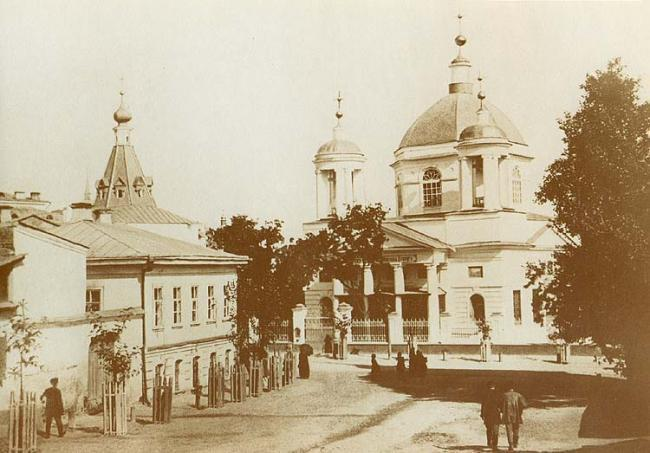
\includegraphics[width=\linewidth]{chast-colebanie-osnov/borichev-tok/nikola_dobry.jpg}
\end{center}

Сего Николу Доброго по проекту Андрея Миленского возводили семь лет. Это здесь, в «Белой гвардии», отпевали мать Турбиных. Тут же действительно служил, до 1930-го, священником Александр Глаголев, друг семьи Булгаковых, венчавший писателя с Таисией Лаппой в Николе Доброго же.

Протоиерей Александр был знатоком в области древнееврейского и арамейского, а всего  ведал восемнадцать языков. Во время известного дела Бейлиса о ритуальном убийстве мальчика, на основании экспертизы Глаголева доказывалась невиновность Бейлиса. 

В 1905 году, во время еврейского погрома, навстречу погромщикам вышли крестным ходом Глаголев с прихожанами Николы Доброго, соединившись с подобным крестным же ходом настоятеля Борисо-Глебской церкви Михаила Едлинского.

В том же году Глаголева избрали ректором Киевской Духовной Академии, однако вскоре с должности сместили, поелику Глаголев, будучи духовным цензором, дозволил печатать книгу, где говорилось про осужденное синодом учение имябожников. Впрочем, Глаголев остался профессором кафедры библейской археологии и еврейского языка.

В 1909 году Глаголев скрестил не меч, но перо с археологом Эртелем, когда тот, усматривая в первых пяти книгах Ветхого Завета учение ненависти к людям, выступил с докладом «Еврейство и Тора». Глаголев же ответил работой «Ветхий Завет и его непреходящее значение в Христианской Церкви».

Пережив на два года храм Доброго Николы, Глаголев умер в 1937-м – по копии акта о смерти, «от уросепсиса и недостаточности сердца» в терапевтическом отделении больницы Лукьяновской тюрьмы, либо прямо в кабинете следователя, уполномоченного IV отделения СПО УГБ лейтенанта госбезопасности Зуса Самойловича Гольдфарба. Спустя еще два года, когда Ежова сменил Берия, сам Гольдфарб был уволен из НКВД за «извращенные формы ведения следствия».

В начале шестидесятых обстоятельства смерти Глаголева и митрополита Константина (Дьякова), которых осенью 1937-го допрашивал Гольдфарб, вызвали у «органов» много вопросов. И уже сам допрашиваемый Гольдфарб многое не мог припомнить. 

Остальные прямо или косвенно причастные к событиям, приведшим к гибели Глаголева и Дьякова, оказались уже вне досягаемости.

Начальник 4-го отдела УГБ НКВД УССР Аркадий (Ар\-он) Хатеневер в 1940 году – расстрелян за нарушение социалистической законности. Калужский Соломон Давыдович, бывший заместитель начальника следственной части НКВД УССР – уволен в 1940 году «за невозможностью дальнейшего использования на работе», в 43-м умер. Клопотнюк Николай Сергеевич, инспектор отдела резервов НКВД УССР, умер в 54-м. Нагорный Иван Григорьевич, заместитель коменданта НКВД УССР, пропал без вести в 1942. Обвинители становились обвиняемыми, а осуждающие судимыми.

Сын Александра Глаголева, Алексей, прежний студент студент физико-математического факультета Киевского университета, был настоятелем соседней, Покровской церкви. Он считается «праведником мира» за укрытие евреев от расстрелов в Бабьем яру. Впрочем, он помогал не только евреям. Выдавал людям справки о том, что те служат при церкви, чтобы уберечь их от угона в Германию. Принимал под свой кров, доставал поддельные метрики.

\begin{center}
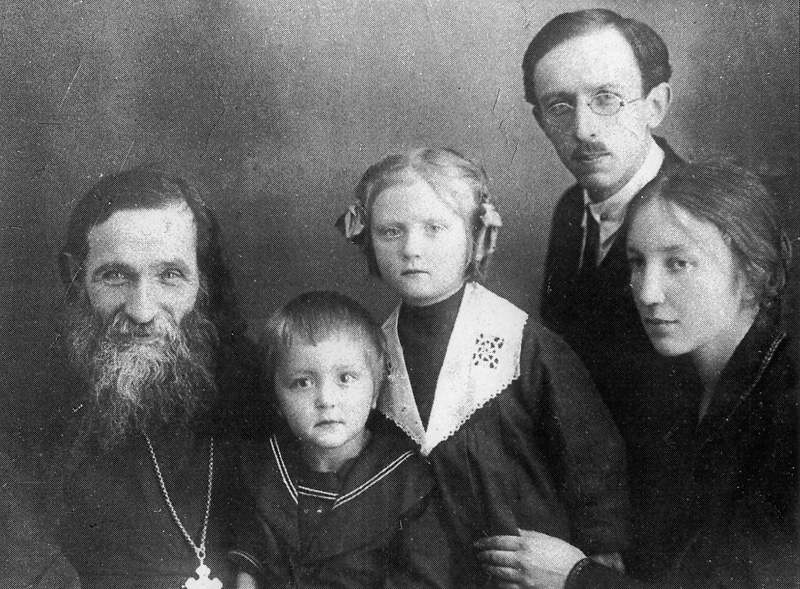
\includegraphics[width=\linewidth]{chast-colebanie-osnov/borichev-tok/glagol-01.jpg}
\end{center}

На этом снимке – Александр Глаголев (слева) с семьей сына Алексея (справа).

После того, как старших Глаголевых в 1932 выгнали из собственного дома\footnote{Тогда имел адрес Покровская, 6.}, Александр с супругой Зинаидой поселились под лестницей в колокольне при храме Николы Доброго. Колокольня тогда именовалась Свято-Варваринской церковью, туда после сноса в 1934-м Борисоглебской церкви\footnote{До революции, Едлинский на пожертвования поставил при церкви четырехэтажный дом, где устроил детский сад (первый в Киеве) для тех ребят, чьи матери нанимались на поденную работу. Там же разместил приходскую школу, приют, кухню и столовую. Сам же ходил в дырявой соломенной шляпе. Лечил пьяниц. А чтобы просящие под церковью не пропивали подаяние, придумал следующее. Прихожане покупали в храме особые купоны на питание в столовой, и наделяли ими нищих. Попутно Едлинский преподавал в Киевской семинарии, коммерческом училище и частной женской гимназии.} перешел служить упомянутый ранее Михаил Едлинский, покуда Николу Доброго не закрыли в 34-м. Глаголев и Едлинский перевелись тогда в Набережно-Никольскую. Двумя годами позже умерла жена Глаголева и была похоронена на Щекавице. После ее смерти Глаголев, когда в гости приходили внуки, много плакал. 

Едлинского расстреляли осенью 1937-го по статьям 54-10 и 54-11 УК УССР\footnote{Антисоветская агитация, участие в контрреволюционной организации.}. Погребен в общей могиле на Лукьяновском кладбище. Та же участь постигла прах Александра Глаголева. Родичи долгое время, до 1944-го не знали про кончину. Передачи в тюрьме принимали до мая 1941 года. Носите, люди добрые!

А за два десятка лет до того, в другом, литературном мире, верно при Булгакове, состоялась беседа:

\begin{quotation}
Ветви в церковном дворе закрыли и домишко священника. Казалось, что сейчас же за стеной тесного кабинетика, забитого  книгами,  начинается  весенний, таинственный спутанный лес. Город по-вечернему глухо шумел, пахло сиренью.

 – Что сделаешь, что сделаешь, – конфузливо  забормотал священник.  (Он всегда конфузился, если приходилось беседовать с людьми.) – Воля божья.

 – Может, кончится  все  это  когда-нибудь?  Дальше-то  лучше  будет?  – неизвестно у кого спросил Турбин.

Священник шевельнулся в кресле.

 – Тяжкое, тяжкое время, что говорить, – пробормотал он, – но унывать-то не следует...

Потом вдруг наложил белую руку, выпростав ее из темного рукава ряски, на пачку книжек и раскрыл верхнюю, там, где она была заложена  вышитой цветной закладкой.

 – Уныния допускать нельзя, – конфузливо, но как-то  очень  убедительно проговорил он. – Большой грех – уныние... Хотя кажется мне, что испытания будут еще. Как же, как же, большие испытания, – он говорил все увереннее.

- Я последнее время все, знаете ли, за книжечками сижу, по специальности, конечно, больше все богословские...

Он приподнял книгу так, чтобы последний свет из окна упал на  страницу, и прочитал:

 – «Третий ангел вылил чашу свою в реки и  источники  вод;  и  сделалась кровь».
\end{quotation}

Пути его с Булгаковым к осени 37-го разошлись. В Москве писатель правит «Мастера и Маргариту», с расчетом напечатать – тогда же рождается это название. Готовит к постановке «Бег» и прекращает писать «Театральный роман». Другая жизнь.

При церкви когда-то был сад, в нем стоял дом Глаголева, потом вырубили и сад, и дом снесли, а много лет назад дети с Андреевского спуска играли в том саду, дети Глаголева донашивали вещи детей Булгаковых, а маленького Глаголева Алексея – Лёсика – на санках возили наверх к Варваре Михайловне Булгаковой, матери Миши, на уроки – так придумал старший Глаголев, чтобы поддержать вдову денежно. Лёсик вырос, стал священником Покровской церкви, при Хрущеве ее обратили в склад поломанных телевизоров, и тогда умер Алексей.

Следующий снимок я сделал с Боричева Тока в 2011 году. Вперед уходит прежний Боричев переулок, ныне упраздненный. Справа – желтая колокольня церкви Покрова, за нею белеет крыло школы номер 100 – то самое, где стояла церковь Николы Доброго. 

Справа от желтой колокольни – старый контрактовый дом, его на этой фотографии не видно. А левее школьного крыла, из-за двухэтажного розоватого домика причта, выглядывает белая с темно-серым куполом – колокольня Николы Доброго, последнее жилище Александра Глаголева.

\vspace*{\fill}

\begin{center}
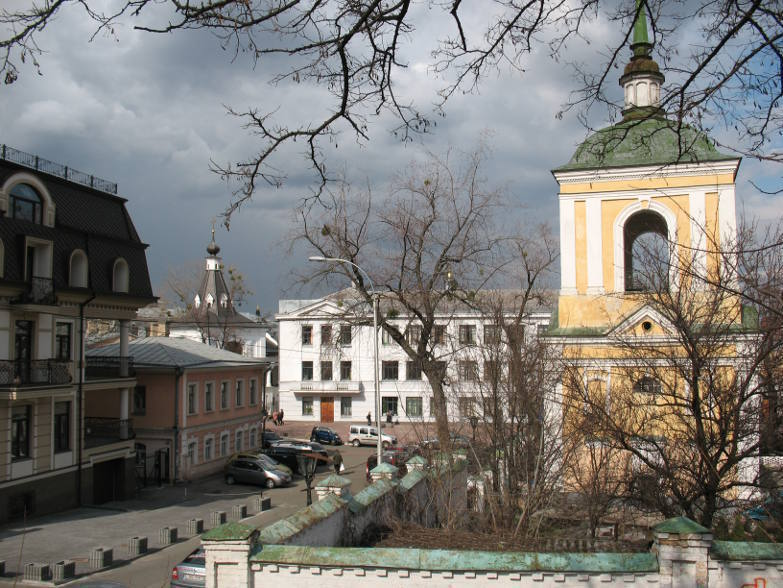
\includegraphics[width=\linewidth]{chast-colebanie-osnov/borichev-tok/pok01-1.jpg}
\end{center}

\vspace*{\fill}


На следующих снимках поглядим, что оказалось бы у нас за спиной в 2005 году. Два дома рядом, 23/3 и 25. Последний пригляден, он с памятной табличкой, о нем заботятся, окна нижнего этажа оковали узорчатой решеткой. 23/3 стоит заброшкой, с каждым часом разрушаясь. 

Вид на юго-восток, слева будут одноэтажки – памятники архитектуры, да церковь Покрова. Как же сильно вросли дома в землю по сравнению со старым Боричевым Током, живым и людным! 
 
\newpage
\vspace*{\fill}
\begin{center}
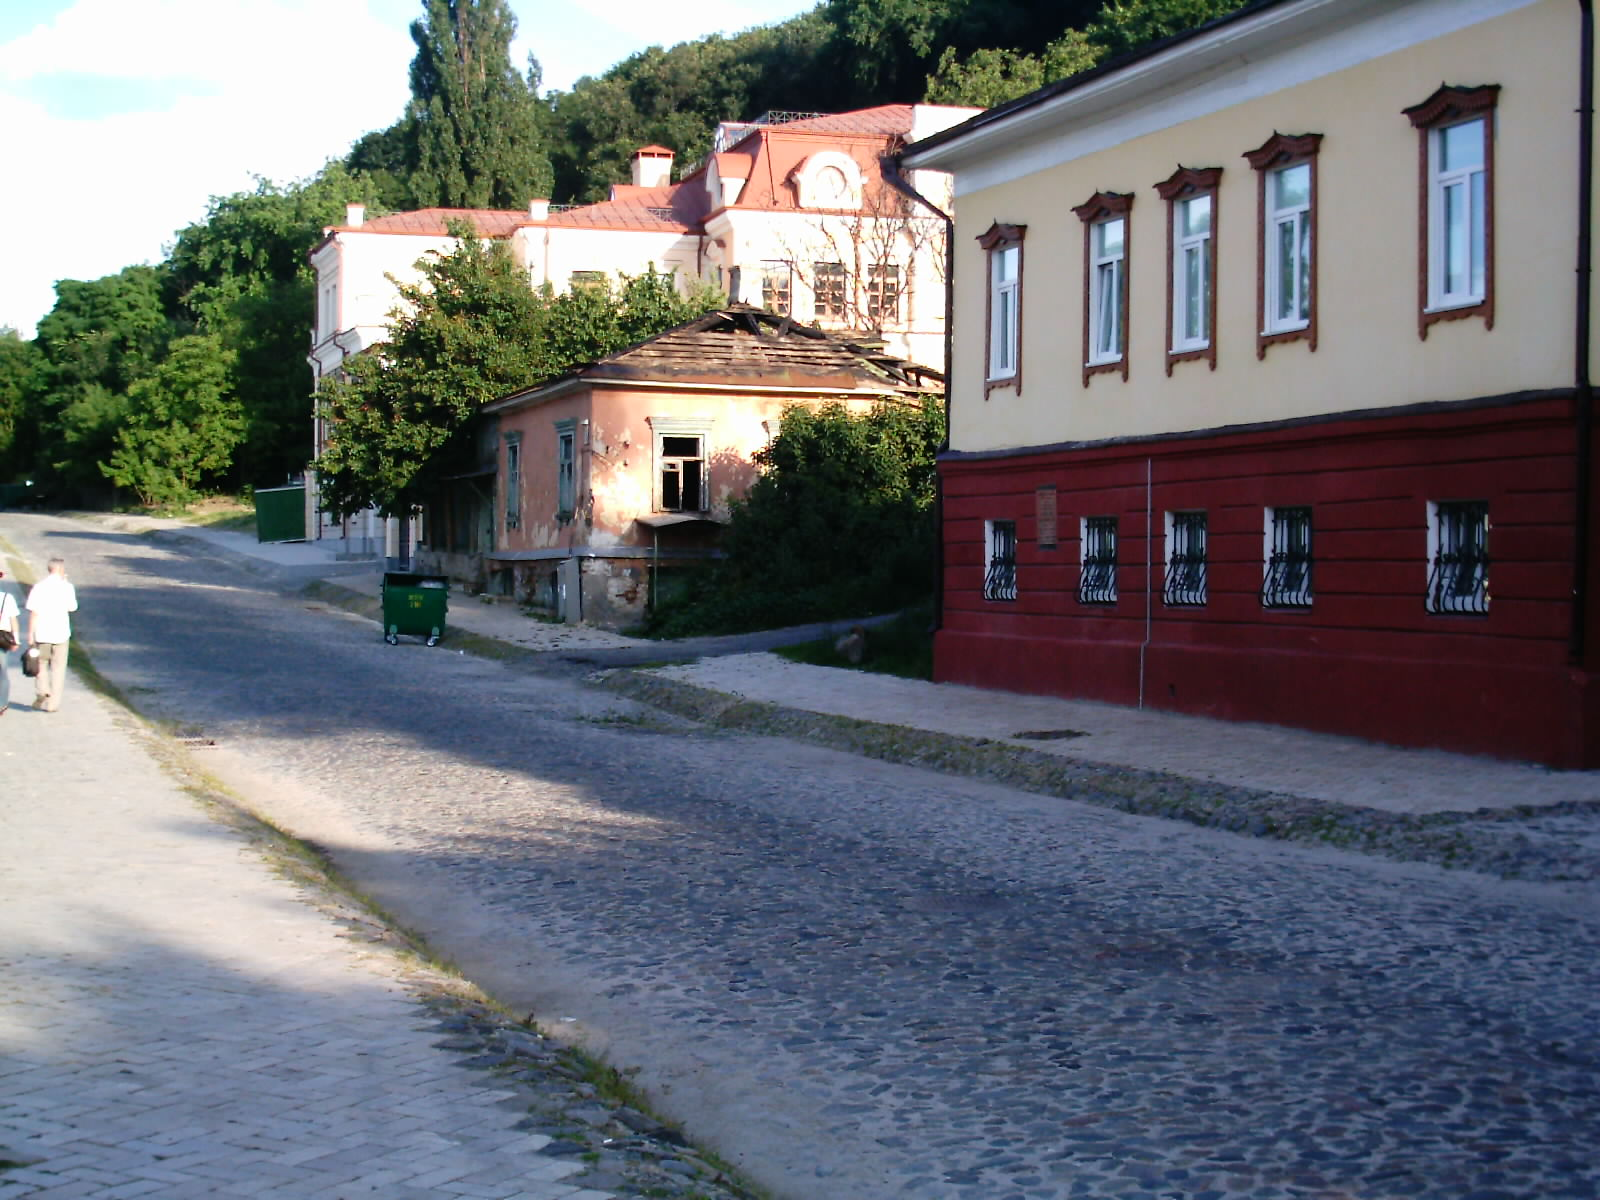
\includegraphics[width=0.95\linewidth]{chast-colebanie-osnov/borichev-tok/bort-imag0001.jpg}
\end{center}

\begin{center}
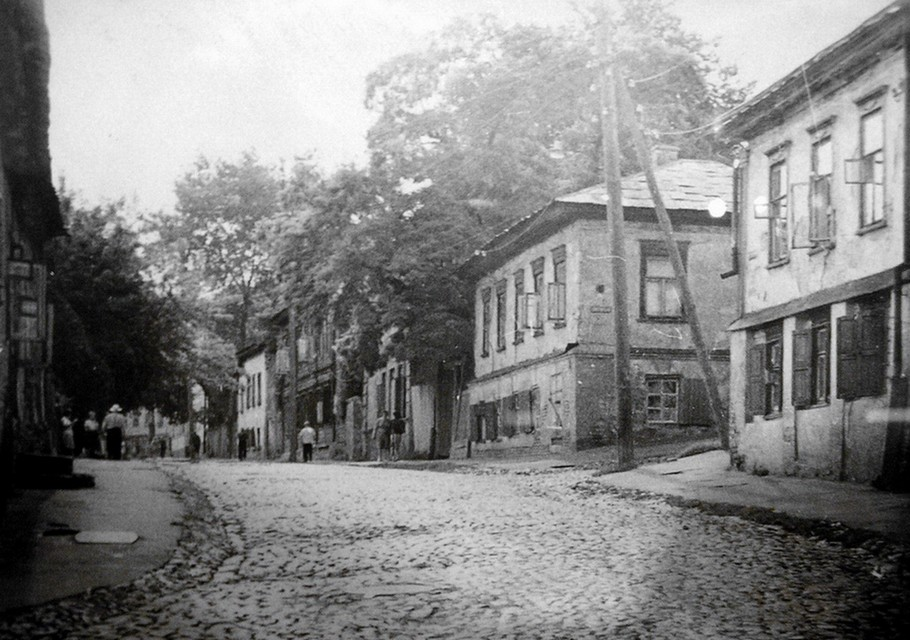
\includegraphics[width=0.95\linewidth]{chast-colebanie-osnov/borichev-tok/bor-tok-23.jpg}
\end{center}
\vspace*{\fill}
\newpage

Вот 23-й номер ближе, и развалины неведомого мне номера, дальше на юго-восток по нечетной стороне. Ветхий, из дранки и дерева, прятался он в глубине.

\begin{center}
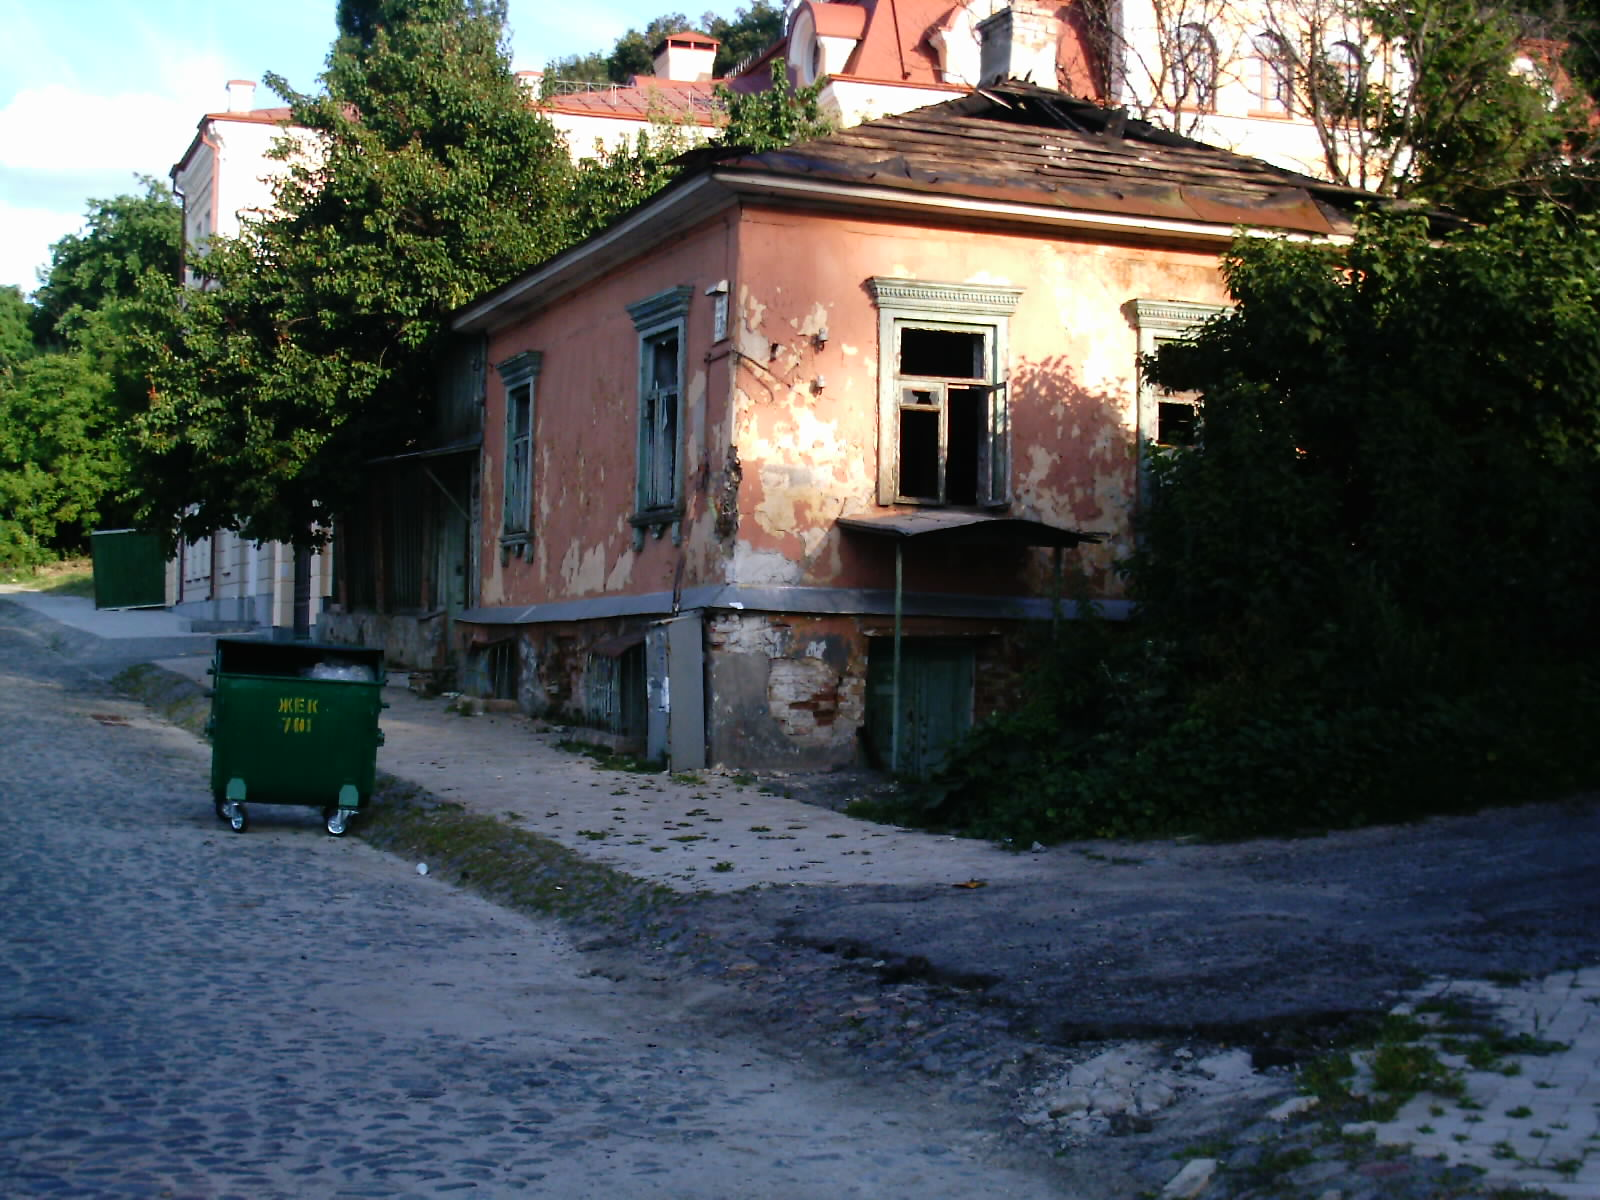
\includegraphics[width=0.96\linewidth]{chast-colebanie-osnov/borichev-tok/bort-imag0004.jpg}
\end{center}

\begin{center}
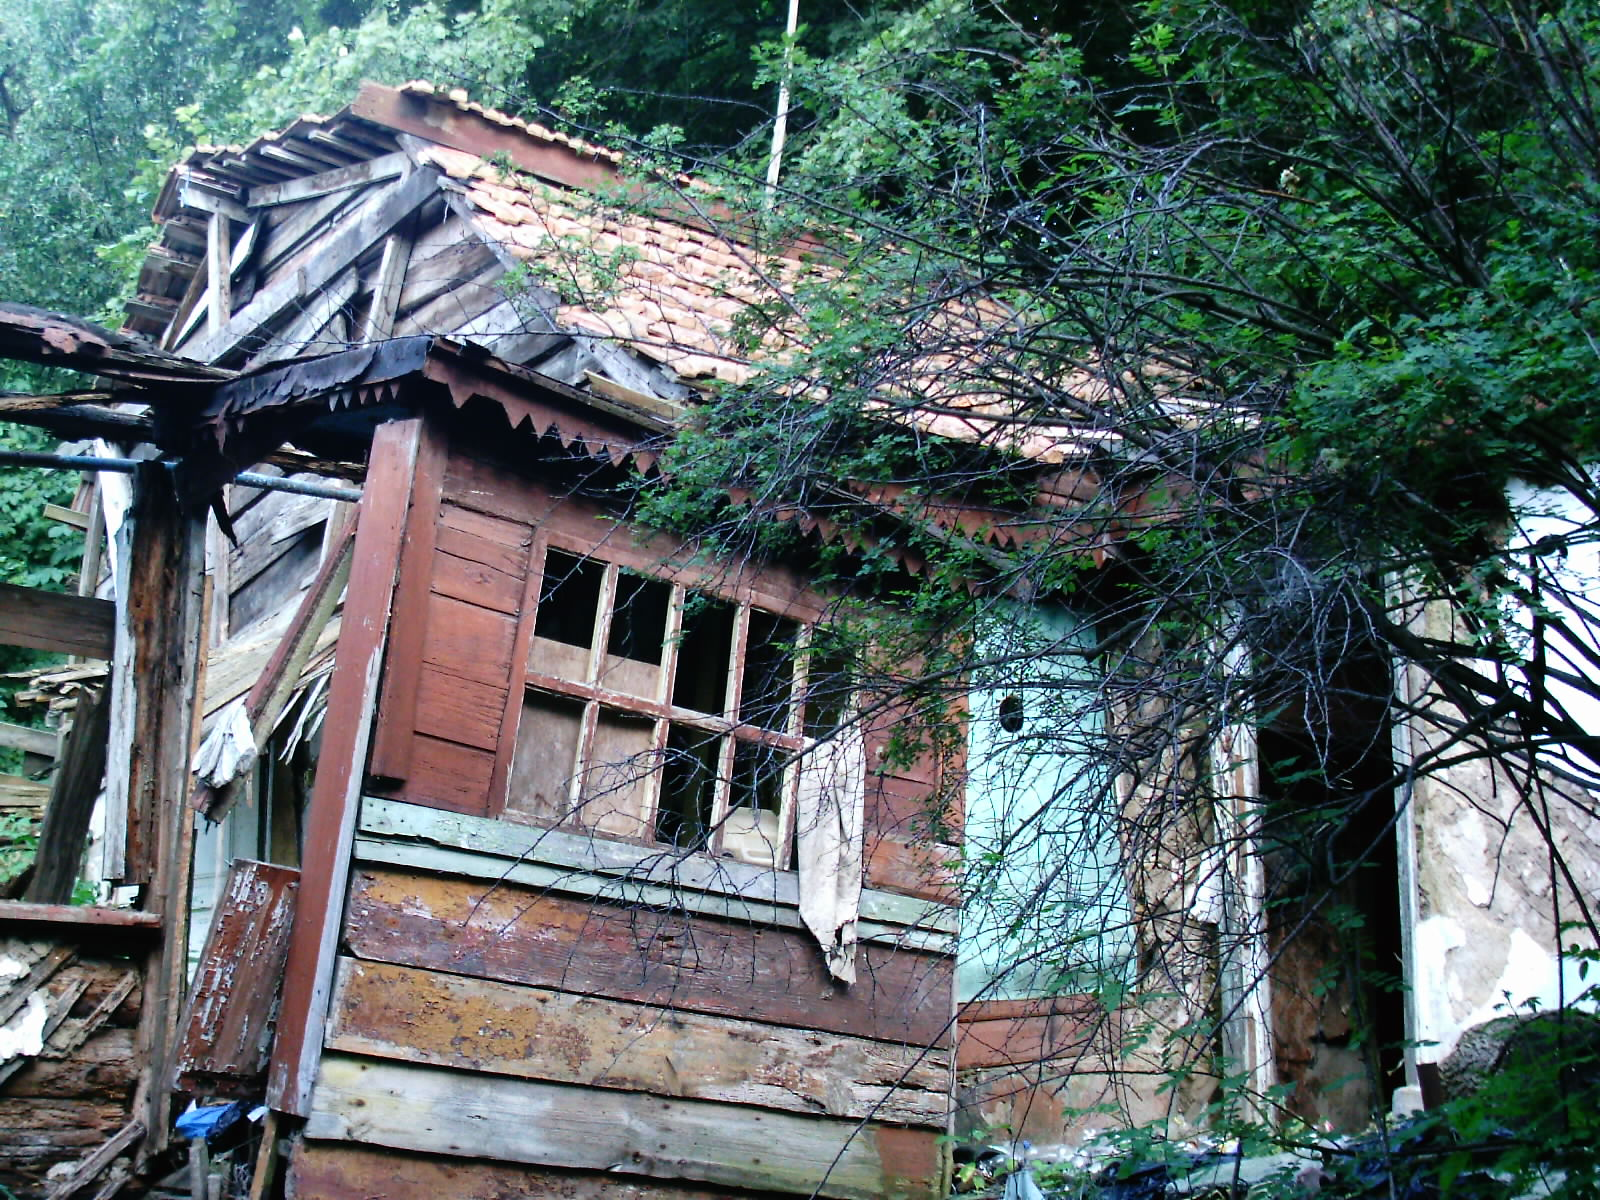
\includegraphics[width=0.96\linewidth]{chast-colebanie-osnov/borichev-tok/bort-imag0011.jpg}
\end{center}

\newpage

\begin{center}
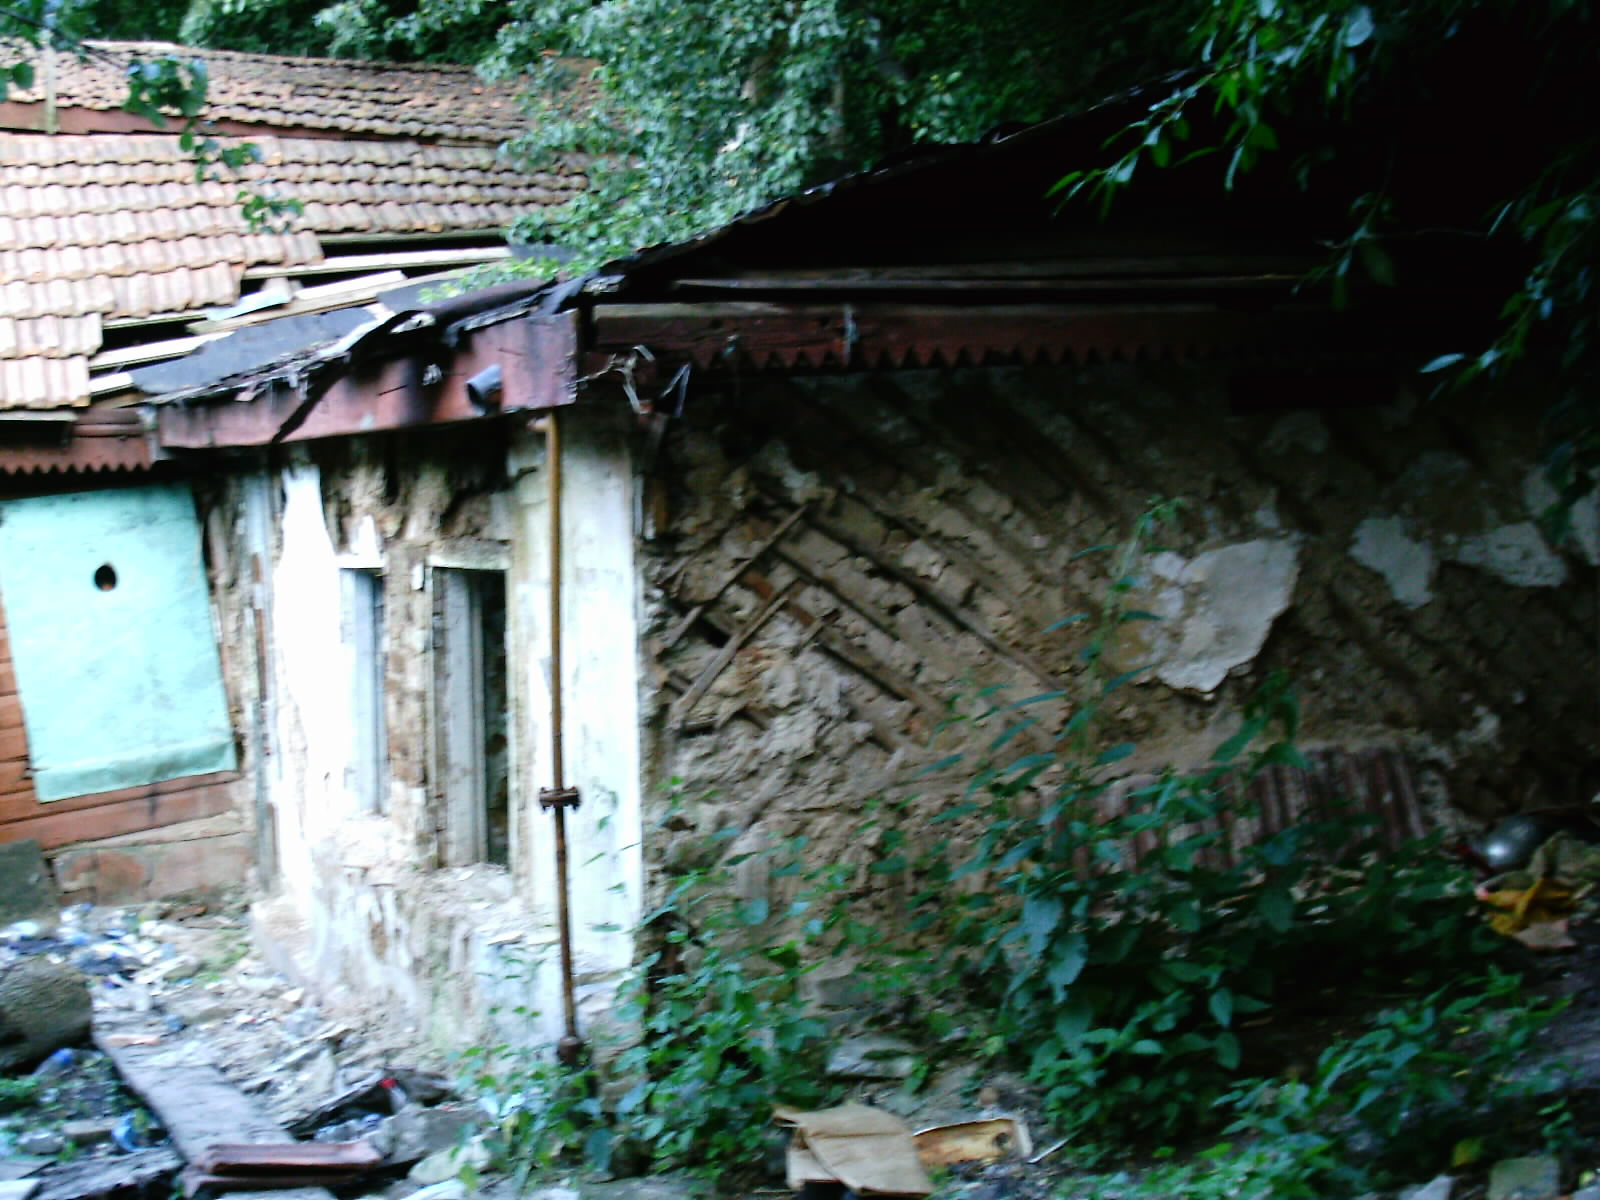
\includegraphics[width=\linewidth]{chast-colebanie-osnov/borichev-tok/bort-imag0023.jpg}
\end{center}

\begin{center}
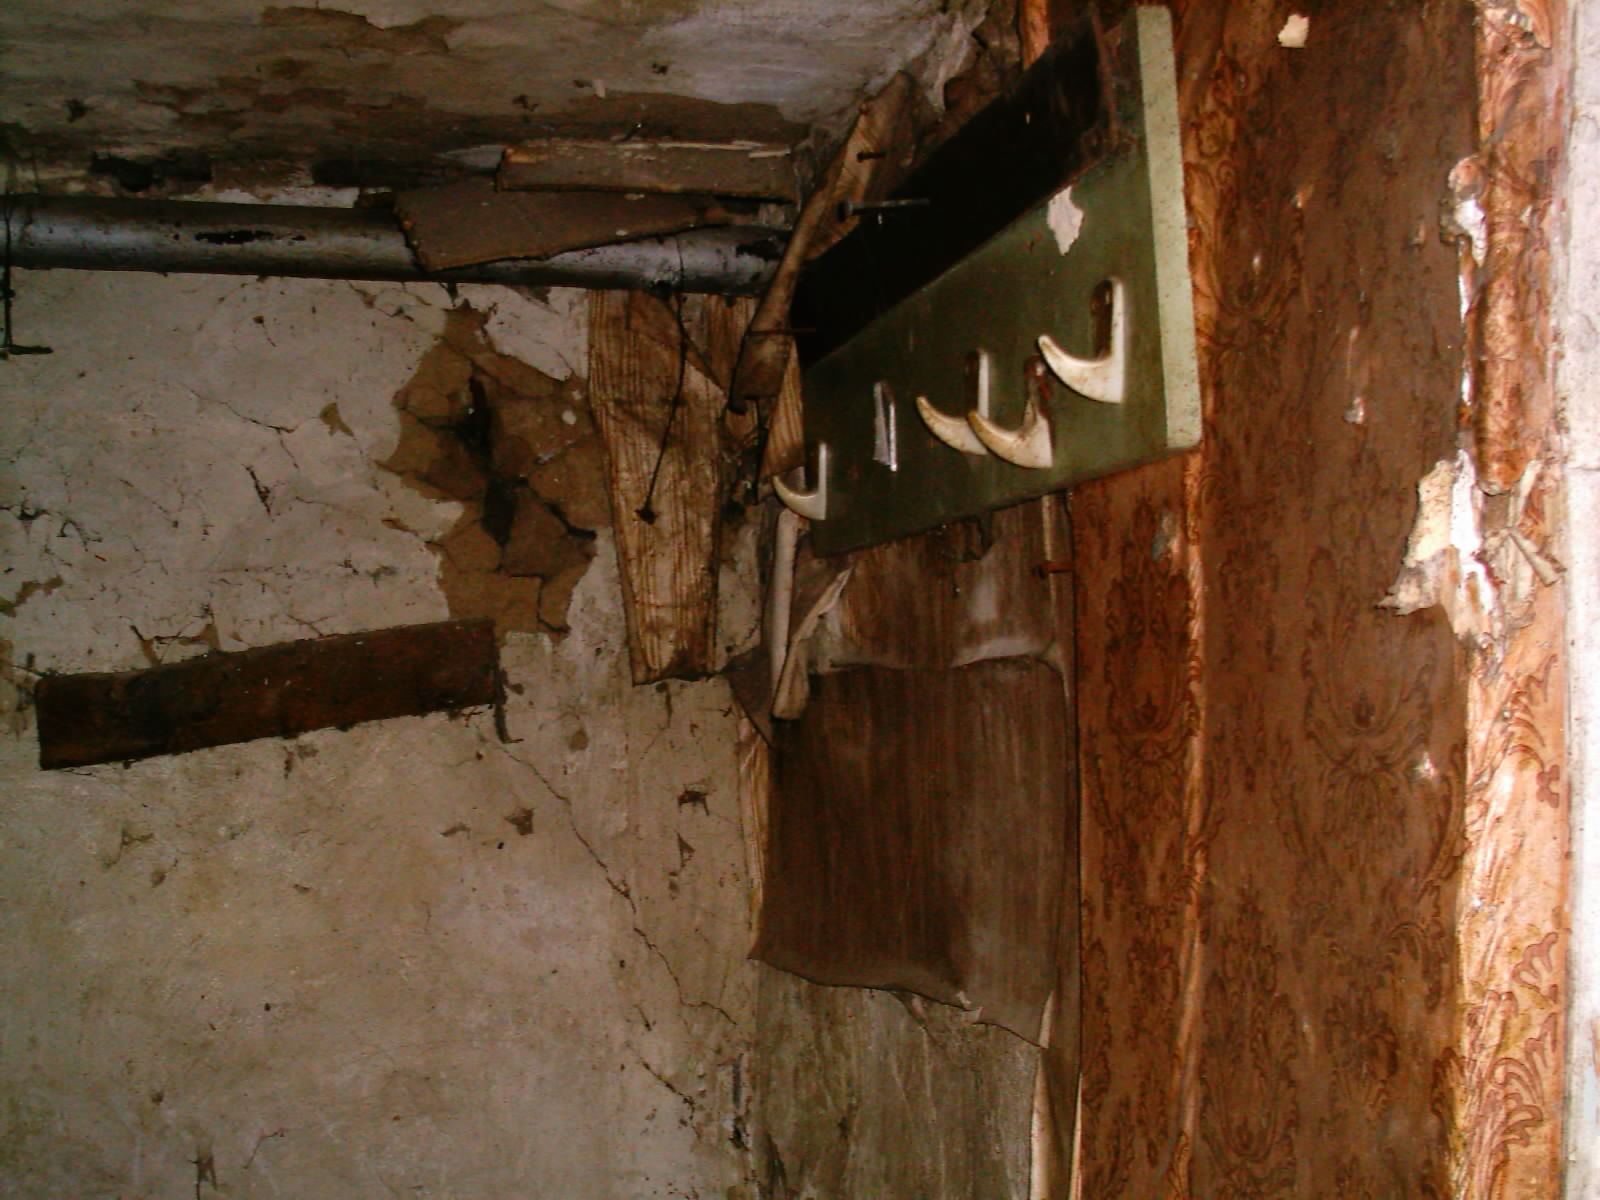
\includegraphics[width=\linewidth]{chast-colebanie-osnov/borichev-tok/bort-imag0033.jpg}
\end{center}

Крючки на вешалке были прикручены шурупами неровно, чехардой. От влажной одежды обои сырели, шли пузырями, какое-то время их подклеивали кусками. Заходил человек, пристраивал сюда пальто, а шляпу – тогда много носили шляпы – непременно цеплял на торчащий сверху здоровенный гвоздь. Должно быть помнит эта вешалка одежду гостей, как нагромождались тут один на другой плащи, и как постепенно освобождалась она, когда гости прощались и уходили. Свобода значит одиночество.
 
И еще дореволюционные рисунок и фотографии. Вид с перекрестка улиц Покровской и Андреевской – вот она пошла вперед, упираясь в Боричев Ток под Андреевской церковью, в склон, куда доходила граница сада Кучинской. За спиной у нас оказывается, по правую руку, через еще одно здание, «старый контрактовый дом», то бишь сотая школа.

С течением лет исчезают и появляются здания, меняется растительность. Не имея точных датировок (кроме фото номер 2, его в 1852 сделал Роджер Фентон), я расставил картинки по возрастанию времени. Оба дома справа на последнем снимке стоят по сей день (номера 2 и 1 на Покровской). Часть склона под Андреевской церковью уже застроена новыми домами на Боричевом Току, много деревьев вырублено, старые здания снесены, участки скрыты за строительными заборами. Дорога, опоясывающая сам пригорок с церковью, сохранилась.


%С течением лет исчезают и появляются здания, меняется растительность. Не имея точных датировок, я расставил картинки по возрастанию времени. Оба дома справа на последнем снимке стоят по сей день (номера 2 и 1 на Покровской). Часть склона под Андреевской церковью уже застроена новыми домами на Боричевом Току, много деревьев вырублено, старые здания снесены, участки скрыты за строительными заборами. Дорога, опоясывающая сам пригорок с церковью, сохранилась.


\begin{center}
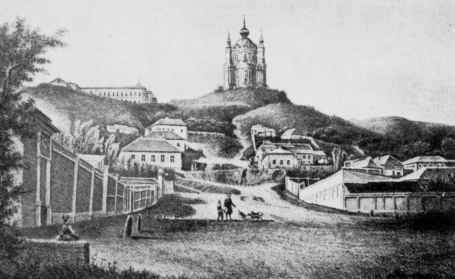
\includegraphics[width=0.96\linewidth]{chast-colebanie-osnov/borichev-tok/kuch03.jpg}
\end{center}

\newpage

\vspace*{\fill}

\begin{center}
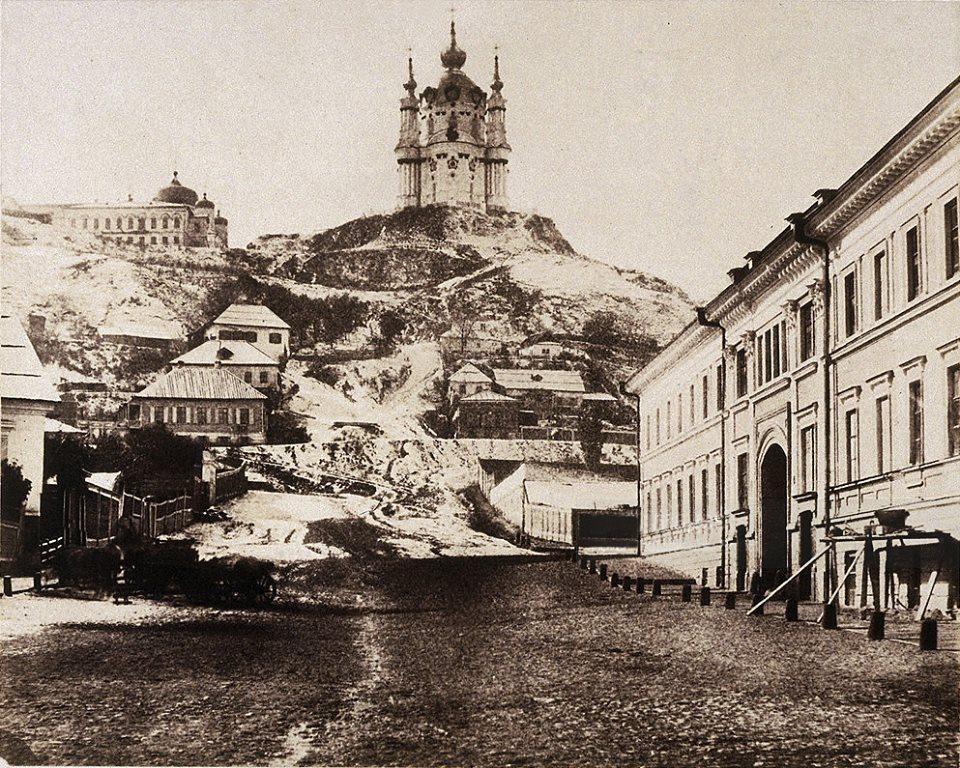
\includegraphics[width=\linewidth]{chast-colebanie-osnov/borichev-tok/kuch04-02.jpg}
\end{center}

\begin{center}
\includegraphics[width=\linewidth]{chast-colebanie-osnov/borichev-tok/\myimgprefix kuch07.jpg}
\end{center}
\vspace*{\fill}

\newpage

\begin{center}
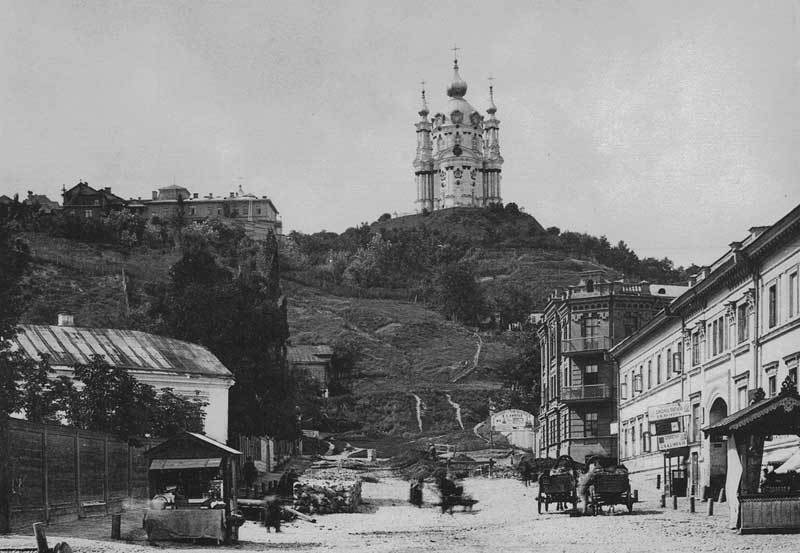
\includegraphics[width=\linewidth]{chast-colebanie-osnov/borichev-tok/kuch02.jpg}
\end{center}

